\documentclass[twocolumn, linenumbers]{aastex701}
\usepackage{tablefootnote}
\usepackage{hyperref}
\usepackage{amsmath}
\usepackage{color}

\newcommand{\fixme}[1]{{\color{red}#1}}

\begin{document}

\title{Unique spectropolarimetric properties of FRBs codetected by CHIME/FRB and DSA-110}
\shorttitle{CHIME/FRB and DSA-110 codetected FRBs}

\author{CHIME/FRB and DSA-110 Collaboration members}
\affiliation{ }
\email{ }


\begin{abstract}
We present spectropolarimetric analysis of twelve apparently non-repeating fast radio bursts (FRBs) that are codetected by CHIME/FRB and DSA-110. Jointly leveraging the data from both observatories, we obtain broadband spectral coverage ($400-1530$~MHz) for these FRBs, and constrain subtle propagation effects in their polarized spectra. We find that the linear polarization fraction in three FRBs decreases with increasing frequency. This spectral signature is commonly observed in pulsars, in which the mixing of two polarized, orthogonal propagation modes causes depolarization at high frequencies; we therefore interpret our results as evidence for a magnetospheric FRB emission process in these systems. Seven FRBs show evidence of decreasing linear polarization fraction with decreasing frequency, consistent with spectral depolarization due to multipath propagation in the source environment. We also report $\geq3\sigma$ detections of positive correlations between the extent of depolarization, amplitude of Faraday rotation measure, and scattering timescale in depolarizing FRBs, implying that all three arise from the same media. The prevalence of depolarization in our sample suggests that inhomogeneous environments surrounding FRB sources are more common than previously expected. In two FRBs, we measure a decrease in the polarization angle (PA) variability with decreasing frequency, as would be expected from amplified scattering of the signal at low frequencies. From this result, we identify a systematic bias towards detecting a disproportionately high fraction of constant PA profiles in current low-frequency (e.g., $400-800$~MHz) FRB surveys.
\end{abstract}

\keywords{Radio bursts (1339) --- Radio transient sources (2008) --- Polarimetry (1278)}


\section{Introduction} \label{sec:intro}
The physical origins of, and emission mechanisms for, fast radio bursts \citep[FRBs; micro- to millisecond duration, coherent radio transients, mostly from extragalactic distances][]{2007Sci...318..777L} remain elusive. The association of one FRB with a Galactic magnetar \citep[FRB~200428;][]{2020Natur.587...54C, 2020Natur.587...59B}, and spectropolarimetric properties suggestive of an emission region near the surface of a rapidly rotating compact object \citep[FRB~20221022A;][]{2025Natur.637...43M, 2025Natur.637...48N}, potentially point towards FRB emission originating from the magnetospheres of magnetars. However, the specific origins of most FRBs \citep[i.e., over 4500;][]{FRBCollaboration_2026_arXiv} remain unresolved, and it is not clear whether all FRBs share a common origin or emission mechanism.

Spectropolarimetric properties of FRBs provide key insights into both the FRB emission process and their source environments \citep[e.g.,][]{2024ApJ...968...50P, Sherman_2024_ApJ, Scott_2025_PASA}. The intrinsic linear and circular polarization fractions ($L/I$ and $|V|/I$, respectively) of FRB signals can help to constrain the type of emission mechanism responsible for their production \citep[e.g.,][]{2023MNRAS.522.2448Q}. Temporal variability of the polarization position angle (PA) across the burst duration traces our viewing geometry of the FRB emission region over $\lesssim$~ms timescales \citep[often parameterized as the ``rotating vector model'' or ``RVM'' that is applied to radio pulsar emission and to some FRBs, e.g.,][]{1969ApL.....3..225R, 2023MNRAS.520.4801J, 2025Natur.637...43M}. 

As FRBs traverse between their emitting source and Earth, their signals accrue a number of frequency-dependent propagation effects from intersecting plasma. Dispersion of radio signals by electrons along the line of sight (LOS), characterized by the dispersion measure (DM), and Faraday rotation of linearly polarized sources, or rotation measure (RM), are two commonly observed properties that inform the density and magnetic field strength of plasma along FRB LOSs.
\begin{equation}
{\rm{DM}}= \int_{0}^{z} \frac{n_e(z)}{(1+z)} \frac{\mathrm{d}l(z)}{\mathrm{d}z}\mathrm{d}z~\mathrm{pc}~\mathrm{cm}^{-3} \label{eq:DM} \,;
\end{equation}
\begin{equation}
{\rm{RM}} = 0.812 \int_{z}^{0} \frac{n_e(z) B_\parallel(z)}{(1 + z)^2}\frac{\mathrm{d}l(z)}{\mathrm{d}z}\mathrm{d}z~\mathrm{rad}~\mathrm{m}^{-2} \label{eq:RM} \,.
\end{equation}
The electron density ($n_e(z)$) is in units of cm$^{-3}$, the LOS magnetic field strength ($B_\parallel(z)$) is in units of $\mu$G, and $\mathrm{d}l(z)$ is the LOS line element at $z$ in units of pc. In Equation \ref{eq:RM}, we integrate between the emitting source (at $z$) to the observer (at $z=0$), so the RM is positive when the average LOS magnetic field is pointed towards the observer and negative when it is pointed away. Spectral depolarization has also been observed in a handful of (mostly repeating) FRBs \citep{2022Sci...375.1266F, 2025MNRAS.tmp.1894U, 2024ApJ...968...50P, 2026ApJ..1000L..53P}, and it has been attributed to multipath propagation through an inhomogeneous magnetoionic plasma near the source.

There are some additional frequency-dependent polarimetric effects that have been studied in radio pulsars that have rarely, if ever, been reported for FRBs. Observations of some pulsars at $\lesssim 1$~GHz, where scatter broadening of the pulse becomes prominent, show that their PA profiles become flattened due to averaging of PAs from different pulse phases within the scattering tail \citep[e.g.,][]{1972AuJPh..25..759K, 2003A&A...410..253L, 2009MNRAS.392L..60K, 2009MNRAS.396.1559N, 2023RAA....23j4002W}. This effect has been observed for one uniquely bright FRB at $400-800$~MHz, FRB~20250316A, where coherent PA variability of amplitude $\sim 30^\circ$ at $\sim 800$~MHz was largely suppressed by scattering at $\sim 400$~MHz \citep{2025ApJ...989L..48C}. 

A number of studies have observed a decreasing linear polarization fraction with increasing observing frequency in pulsar spectra \citep[e.g.,][]{1973ApJ...179L...7M, 1996A&A...309..481X, 1997ApJ...475..763M, 2008MNRAS.388..261J, 2015A&A...576A..62N}. While there is currently no consensus on the specific mechanism responsible for this phenomenon, most of the proposed models rely on the birefringence of plasma in an extreme magnetized environment, such as the magnetosphere of a neutron star \citep{1975ApJ...196...51R, 1986ApJ...302..138B, 1997ApJ...475..763M, 1998A&A...336..209V}. Other explanations of decreasing linear polarization with increasing frequency in pulsars include superimposed orthogonal polarization modes with different spectral indices \citep{2005MNRAS.359..481K} and incoherent summing of short duration bursts originating near the neutron star surface \citep{2008MNRAS.388..261J}$-$both of which still necessitate a magnetospheric emission process. While one FRB shows a potential increase in linear polarization fraction with decreasing frequency between $400-800$~MHz \citep{2024ApJ...968...50P}, there has been no definitive detection of this effect in FRBs.

Our capacity to measure many of these spectropolarimetric effects depends on both our observing frequency ($\nu$) and bandwidth ($\Delta \nu$). While most current FRB experiments have sufficient frequency coverage to reliably measure DM and RM for most detected bursts, constraining more subtle spectropolarimetric effects, such as those mentioned above, requires low-frequency and wide-band observations that provide a large lever arm in frequency space. The problem is exasperated as most FRB sources do not repeat \citep{2023ApJ...947...83C}, thus necessitating instantaneous broadband observations for a single burst. Uniquely, two of the FRB experiments in the Northern hemisphere, the Canadian Hydrogen Intensity Mapping Experiment FRB Project \citep[CHIME/FRB, observing at $400-800$~MHz;][]{2018ApJ...863...48C} and the Deep Synoptic Array 110 \citep[DSA-110, observing at $1280-1530$~MHz;][]{2024ApJ...967...29L}, overlap significantly in survey footprint and can codetect FRB sources.

In a companion paper (J.~Faber et.~al.~in prep.; hereafter ``paper I''), we introduce a sample of twelve apparently non-repeating FRBs codetected by CHIME/FRB and DSA-110. Here, we leverage the combined bandwidth of the two instruments, together spanning two octaves ($400-1530$~MHz), to conduct a joint spectropolarimetric analysis of this codetected FRB sample. In Section \ref{sec:obs}, we describe our CHIME/FRB and DSA-110 observations and summarize the process of identifying codetected FRBs. We detail our modeling of the $L/I$ and PA profile as a function of frequency in Section \ref{sec:models}. In Section \ref{sec:results}, we describe our resulting model fits to the codetected FRB data, finding complex $L/I$ spectra for 8 FRBs, and PA profiles that flatten at low frequencies for two sources. We interpret our measurements in Section \ref{sec:discussion}, showcasing evidence that some of the FRBs may be emitted in the magnetosphere of neutron stars, and we also discuss the implications of low-frequency flattening in PA profiles as an observational systematic in broader polarimetric population studies of FRBs. We summarize our findings and conclude in Section \ref{sec:conclusions}. 


\section{Observations} \label{sec:obs}
\subsection{CHIME/FRB} \label{sec:obs_chime}
CHIME operates between $400-800$~MHz and, as a transit telescope with no moving parts, it observes the sky above a Declination of $-10$~degrees. The telescope is located at the Dominion Radio Astrophysical Observatory in British Columbia, Canada. The CHIME/FRB system conducts a real-time FRB search on the CHIME data stream \citep[for details, see][]{2018ApJ...863...48C} and records two modes of data for FRB candidates: (i) total intensity data at a time resolution of $0.983$~ms and frequency resolution of $24.4$~kHz (for FRBs with a signal-to-noise $\mathrm{S/N} > 8$) and (ii) full polarization channelized voltage data, or ``baseband data'', at a frequency resolution of $390.625$~kHz and a time resolution of $2.56~\mu\mathrm{s}$ (for $\mathrm{S/N} > 12$).\footnote{The threshold is reduced to $\mathrm{S/N} > 10$ for subsequent bursts from a known repeating FRB source.} The median sky position uncertainty derived from the total intensity data is relatively coarse, $\sim0.2^\circ$, with localization confidence intervals often forming non-Gaussian distributions \citep[for details, see][]{2019ApJ...885L..24C, 2021ApJS..257...59C, FRBCollaboration_2026_arXiv}. However, raw voltage information is preserved for FRBs that exceed the S/N threshold for saving baseband data, allowing for their localizations to be later refined by a S/N-maximizing search over a dense grid of formed beams; the median sky position uncertainty for FRBs with baseband data is $\sim20''$ \citep{Michilli2024}. FRBs discovered by CHIME/FRB are broadcast to the community using a low-latency virtual observatory events (VOEvents) system \citep{2025AJ....169...39A}, which contains burst properties and detection information, for example: time of arrival (TOA; topocentric at CHIME and referenced to $400$~MHz), real-time detection S/N,\footnote{Details of the real-time CHIME/FRB search pipeline are described by \citep{2018ApJ...863...48C}.} sky position, and DM.

To derive polarization data products at $400-800$~MHz for this work, we employ the CHIME/FRB polarization pipeline \citep[for details, see][]{2021ApJ...920..138M, 2024ApJ...968...50P}. The FRB burst envelope temporal limits are identified as the region in which the total intensity is $>20$\% of the peak burst intensity. Stokes $I$, $Q$, $U$, and $V$ spectra are produced by integrating over this burst envelope with uniform weights in time. We apply RM-synthesis \citep{2005A&A...441.1217B} to the FRB Stokes spectra, obtaining a robust RM detection if the peak polarized intensity in Faraday depth space is $>6\sigma$ after applying {\tt RM-CLEAN} \citep{2009A&A...503..409H}. We then apply the QU-fitting algorithm \citep[implemented with a modified version of V1.2 of the {\tt RM-tools} package;][]{2020ascl.soft05003P, 2026arXiv260120092V}, using the default model described by \cite{2021ApJ...920..138M}. This QU-fitting step provides an independent measurement of the FRB RM\footnote{In some cases, instrumental polarization can cause the sign of the RM derived via QU-fitting to be incorrect \citep[see Appendix A by][]{2021ApJ...920..138M}. Thus, we opt to use the RM estimate from RM-synthesis throughout this work. A detailed analysis to mitigate this QU-fitting sign error will be presented in upcoming work by M.~Ng et al.~(in prep.) and in \fixme{\citet{2024ApJ...964..131S}}.}. as well as an estimate of the physical (cable) delay between the two linear polarizations, which can act as a source of contamination between Stokes $U$ and $V$. We then return to the Stokes dynamic spectra, derotate them given the FRB RM, apply a correction based on the measured cable delay term, and integrate over the burst envelope temporal limits to obtain a set of ``corrected'' Stokes $I$, $Q$, $U$, and $V$ spectra that we use for any further analysis.

For any bursts that do not satisfy the $6\sigma$ linearly polarized signal-to-noise criterion, we only measure an upper limit on their $L/I$ averaged across $400-800$~MHz of $6/(\mathrm{S/N}(I))$, where $\mathrm{S/N}(I)$ is the signal-to-noise of the Stokes $I$ signal \citep{2024ApJ...968...50P}.

\subsection{DSA-110} \label{sec:obs_dsa}
The DSA-110 is a radio interferometer located at the Owens Valley Radio Observatory that is designed to detect and precisely localize (to a radius of $\sim$ a few arcseconds) FRBs between $1280-1530$~MHz. The data presented in this work were collected during the science commissioning stage in which the interferometer was comprised of sixty-three, $4.65$~m, antennas, each equipped with dual-linear-polarization receivers that are distributed across a $2.5$~km area \citep{2024ApJ...967...29L}. During commissioning the antenna were pointed at a declination of $71.6^\circ$ with an effective field of view of $10^{\circ}{}^{2}$. An FRB search was conducted at a frequency and time resolution of $30.52$~kHz and $32.768~\mu\mathrm{s}$, respectively, using 48 core antennas while the remaining 15 antennas, with longer baselines, were used to assist in FRB localization \citep{Sherman_2024_ApJ}. Following a real-time detection, candidate positions from the coherent search beams are refined offline by forming interferometric visibilities from the saved voltage data of the core and outrigger antennas, calibrating them using nearby calibrator observations and an NRAO VLA Sky Survey sky model, and imaging the burst with the long-baseline data \citep{2023ApJ...949L...3R}. The sky position is measured by fitting a two-dimensional Gaussian to the deconvolved burst image, yielding typical $90\%$ confidence uncertainties of $\lesssim 2''$ \citep{2024ApJ...967...29L, 2023ApJ...949L...3R}. Full-polarization channelized voltage data are saved for FRB candidates that pass the real-time search trigger \citep{2024ApJ...967...29L}, namely: (i) a detection $\mathrm{S/N} > 8.5$ in any coherent search beam, (ii) no association with strong terrestrial radio-frequency interference, and (iii) $\mathrm{DM} > 50$~pc~cm$^{-3}$ and greater than 75\% of the Galactic DM estimate along the line of sight based on the NE2001 model \citet{2002astro.ph..7156C}. For detailed descriptions of the DSA-110 system and FRB search during science commissioning, see \citep{2023ApJ...949L...3R, 2024ApJ...967...29L}.

Here, we summarize the polarization pipeline, described in detail by \cite{Sherman_2024_ApJ}, that we use to derive polarization data products at $1280-1530$~MHz for this work. First, calibration is applied to reduce the effect of instrumental polarization due to differences in gain (leakage between Stokes $I$ and $Q$) and phase (leakage between Stokes $U$ and $V$; also called ``cable delay'' in Section \ref{sec:obs_chime}) between the two linearly polarized receivers. Two bright radio sources, one with known polarization (3C286; $L/I = 0.095$ at $1400$~MHz) and one unpolarized (3C48; $L/I \lesssim 0.005$), are used to derive a Jones matrix and correct for these instrumental polarization effects. Absolute PAs are estimated by treating the DSA-110 as a single antenna, deriving its elevation and azimuth given the position of the FRB-detecting beam and the detection local sidereal time to estimate the parallactic angle, which is then applied as a correction to the observed PA \citep[for further details regarding the polarization calibration, see Appendices D$-$G by][]{Sherman_2024_ApJ}.

For a given FRB, Stokes spectra are generated by averaging over the temporal extent of the burst, which is determined manually to encompass all components in the case of multi-component bursts. Similar to the CHIME/FRB polarization pipeline, an RM search is conducted on these Stokes spectra using the version of RM-synthesis implemented in the {\tt RM-tools} package \citep{2005A&A...441.1217B, 2020ascl.soft05003P, 2026arXiv260120092V}. Instead of searching for an RM across the entire burst envelope, the linearly polarized signal in the Faraday dispersion function (FDF) is maximized for each time step in the burst, and the resulting time-resolved RMs across the burst are averaged to get a single RM for the burst. If a significant (i.e., linearly-polarized signal to noise exceeding $9\sigma$) is detected, the Stokes dynamic spectra are derotated to correct for the measured RM. Integrating these derotated Stokes spectra across the temporal extent of the FRB then provides the equivalent set of ``corrected'' Stokes $I$, $Q$, $U$, and $V$ spectra at $1280-1530$~MHz that we use for further analysis.


\section{Search for codetected FRBs} \label{sec:obs_codetections}
We identify twelve apparently non-repeating FRBs jointly detected by CHIME/FRB and DSA-110 between 2022 February and 2024 February. Candidate pairs are required to have consistent sky positions and arrival times: after correcting for the inter-site geometric light-travel delay and cold-plasma dispersion to a common reference frequency of $400$~MHz, the timing residuals across the sample are consistent with the combined instrumental uncertainties (median residual $\sim 2$ ms; 1$\sigma$ $\pm 2.5$ ms; paper I). Angular separations between the CHIME/FRB and DSA-110 localizations are consistent to within their uncertainties (albeit $\lesssim$ a few arcminutes) for every burst. Independent dispersion measures estimated at each facility agree where both are well constrained. Each association is additionally vetted by visual comparison of the total-intensity dynamic spectra, including agreement in the number of temporal components across the two bands; the clearest multi-component example is FRB~20220310F, for which the detailed morphology comparison is presented in paper~I. The resulting sample comprises twelve non-repeating, broadband events spanning $262$--$960$~pc~cm$^{-3}$ in DM; spectroscopic host-galaxy redshifts are available for nine bursts, while FRBs~20221203A, 20230325A, and 20240122A lack a confirmed host redshift. Morphology of the codetected bursts along with their scattering timescales, scintillation bandwidths, host-galaxy associations, estimated energies, and an analyses of their foregrounds are reported in paper~I.


\section{Spectropolarimetric modeling} \label{sec:models}
We focus on analyzing the $L/I$ and PA profile of the codetected FRBs as a function of frequency, and we quantify and model their spectral properties based on frequency-dependent polarization effects that have been previously observed in other FRBs and in some radio pulsars. In this work, we do not analyze the circular polarization fraction, $|V|/I$, as CHIME/FRB data suffers from unmodeled instrumental sources of circular polarization that can lead to $|V|/I\sim 20\%$ uncertainties and limit our sensitivity to frequency-dependent circular polarization effects \citep{2021ApJ...920..138M}.

\subsection{Linear polarization} \label{sec:models_li}
We model the observed linear polarization fraction as a function of frequency, $L/I (\nu)$, using three different frameworks, each adding a layer of complexity to describe potential propagation effects arising in foreground magnetoionic plasma. These models are described below and example $L/I (\nu)$ spectra between $400-1530$~MHz for each of the three scenarios, using some fiducial model parameters, are presented in Figure \ref{fig:li_models}. The models are meant to be representative but they are not the only possible models to describe these physical phenomena. Nonetheless, they adequately describe the data, suggesting that more complex modeling is not justified in the present work.

\begin{figure*}
    \centering
    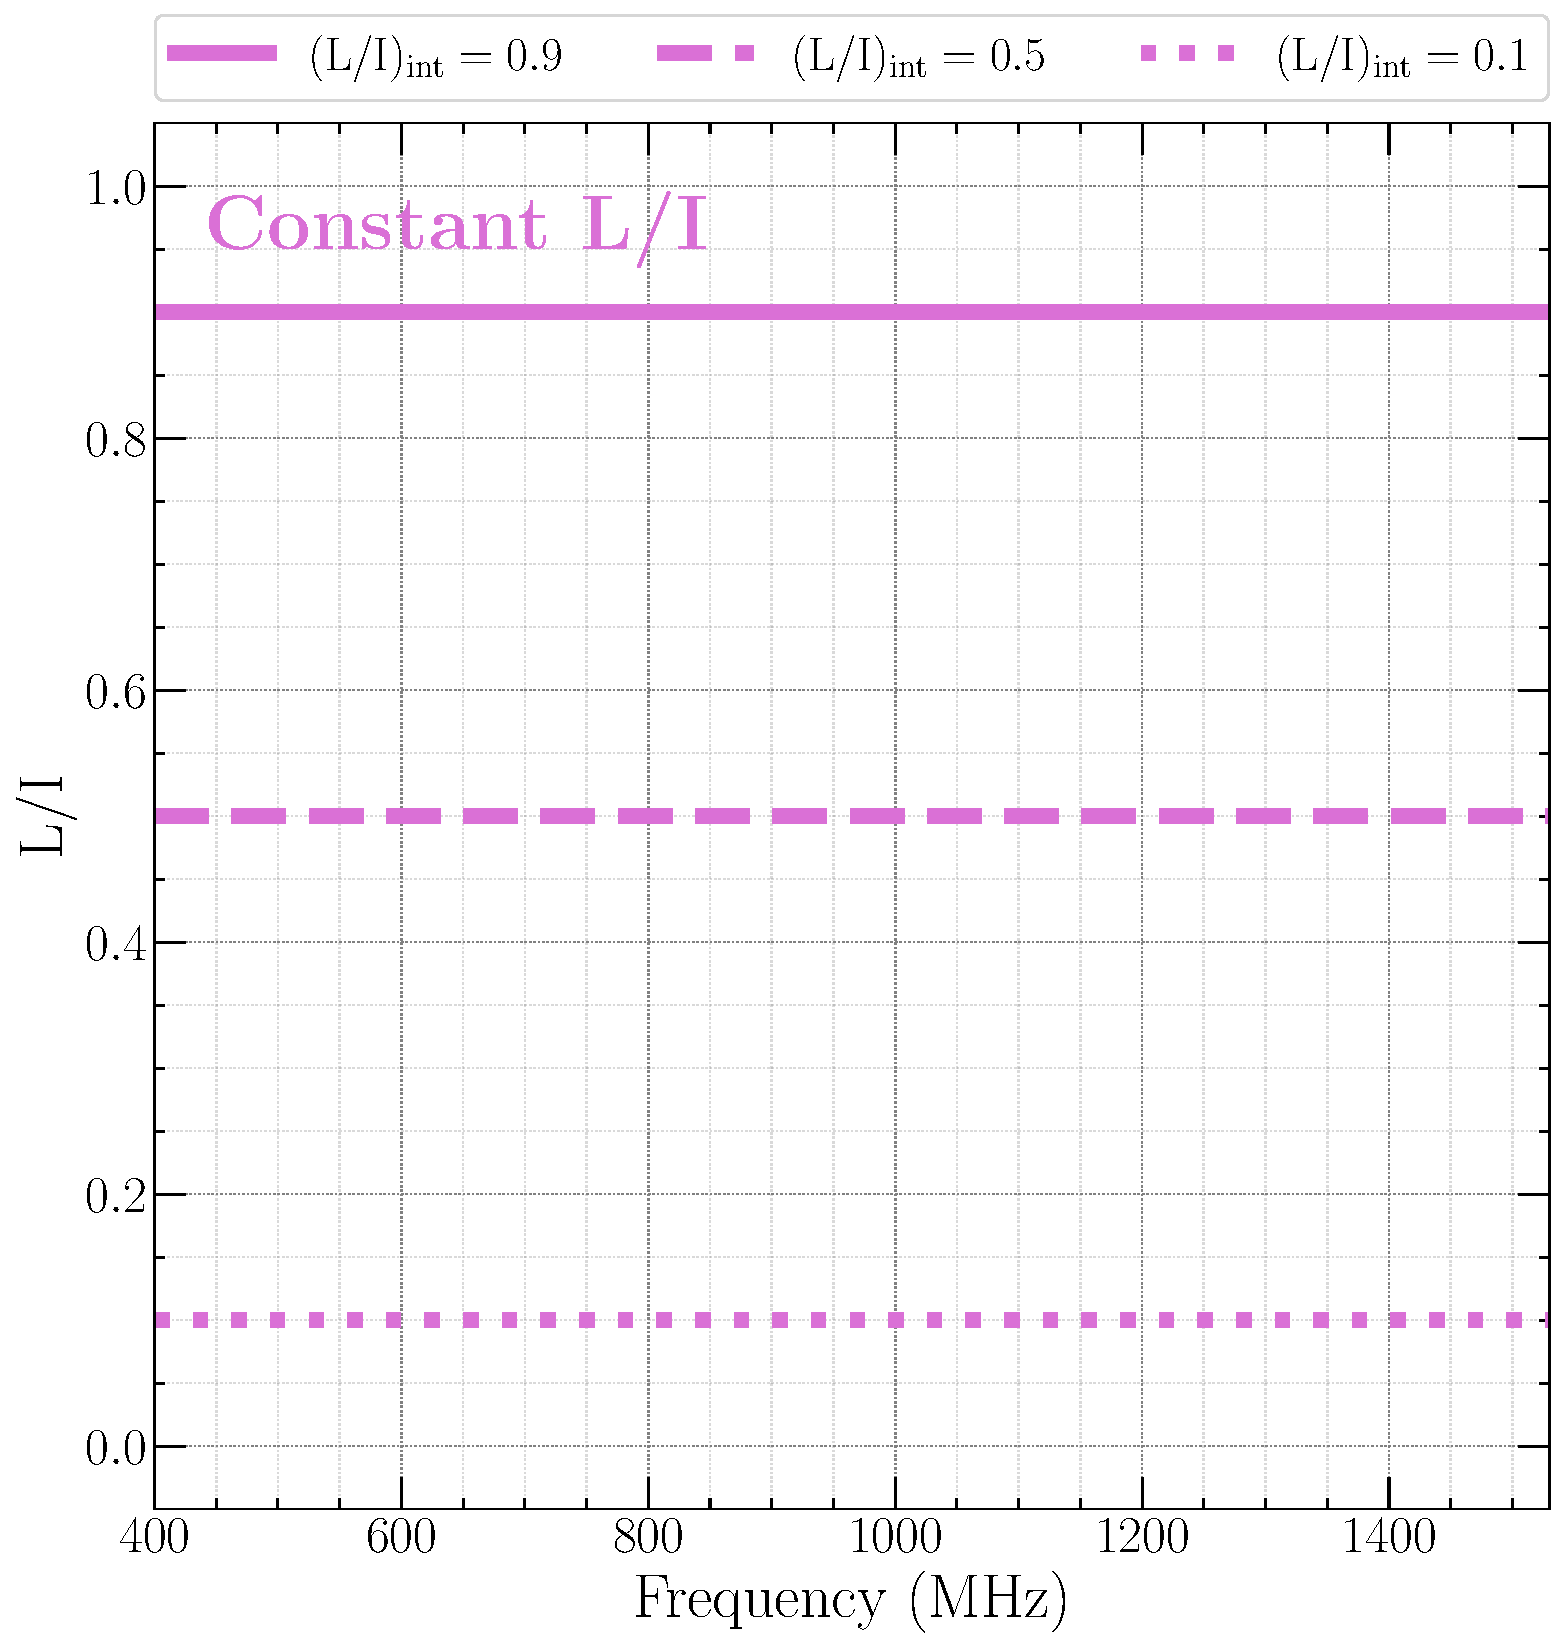
\includegraphics[width=0.329\textwidth]{model_1.pdf}
    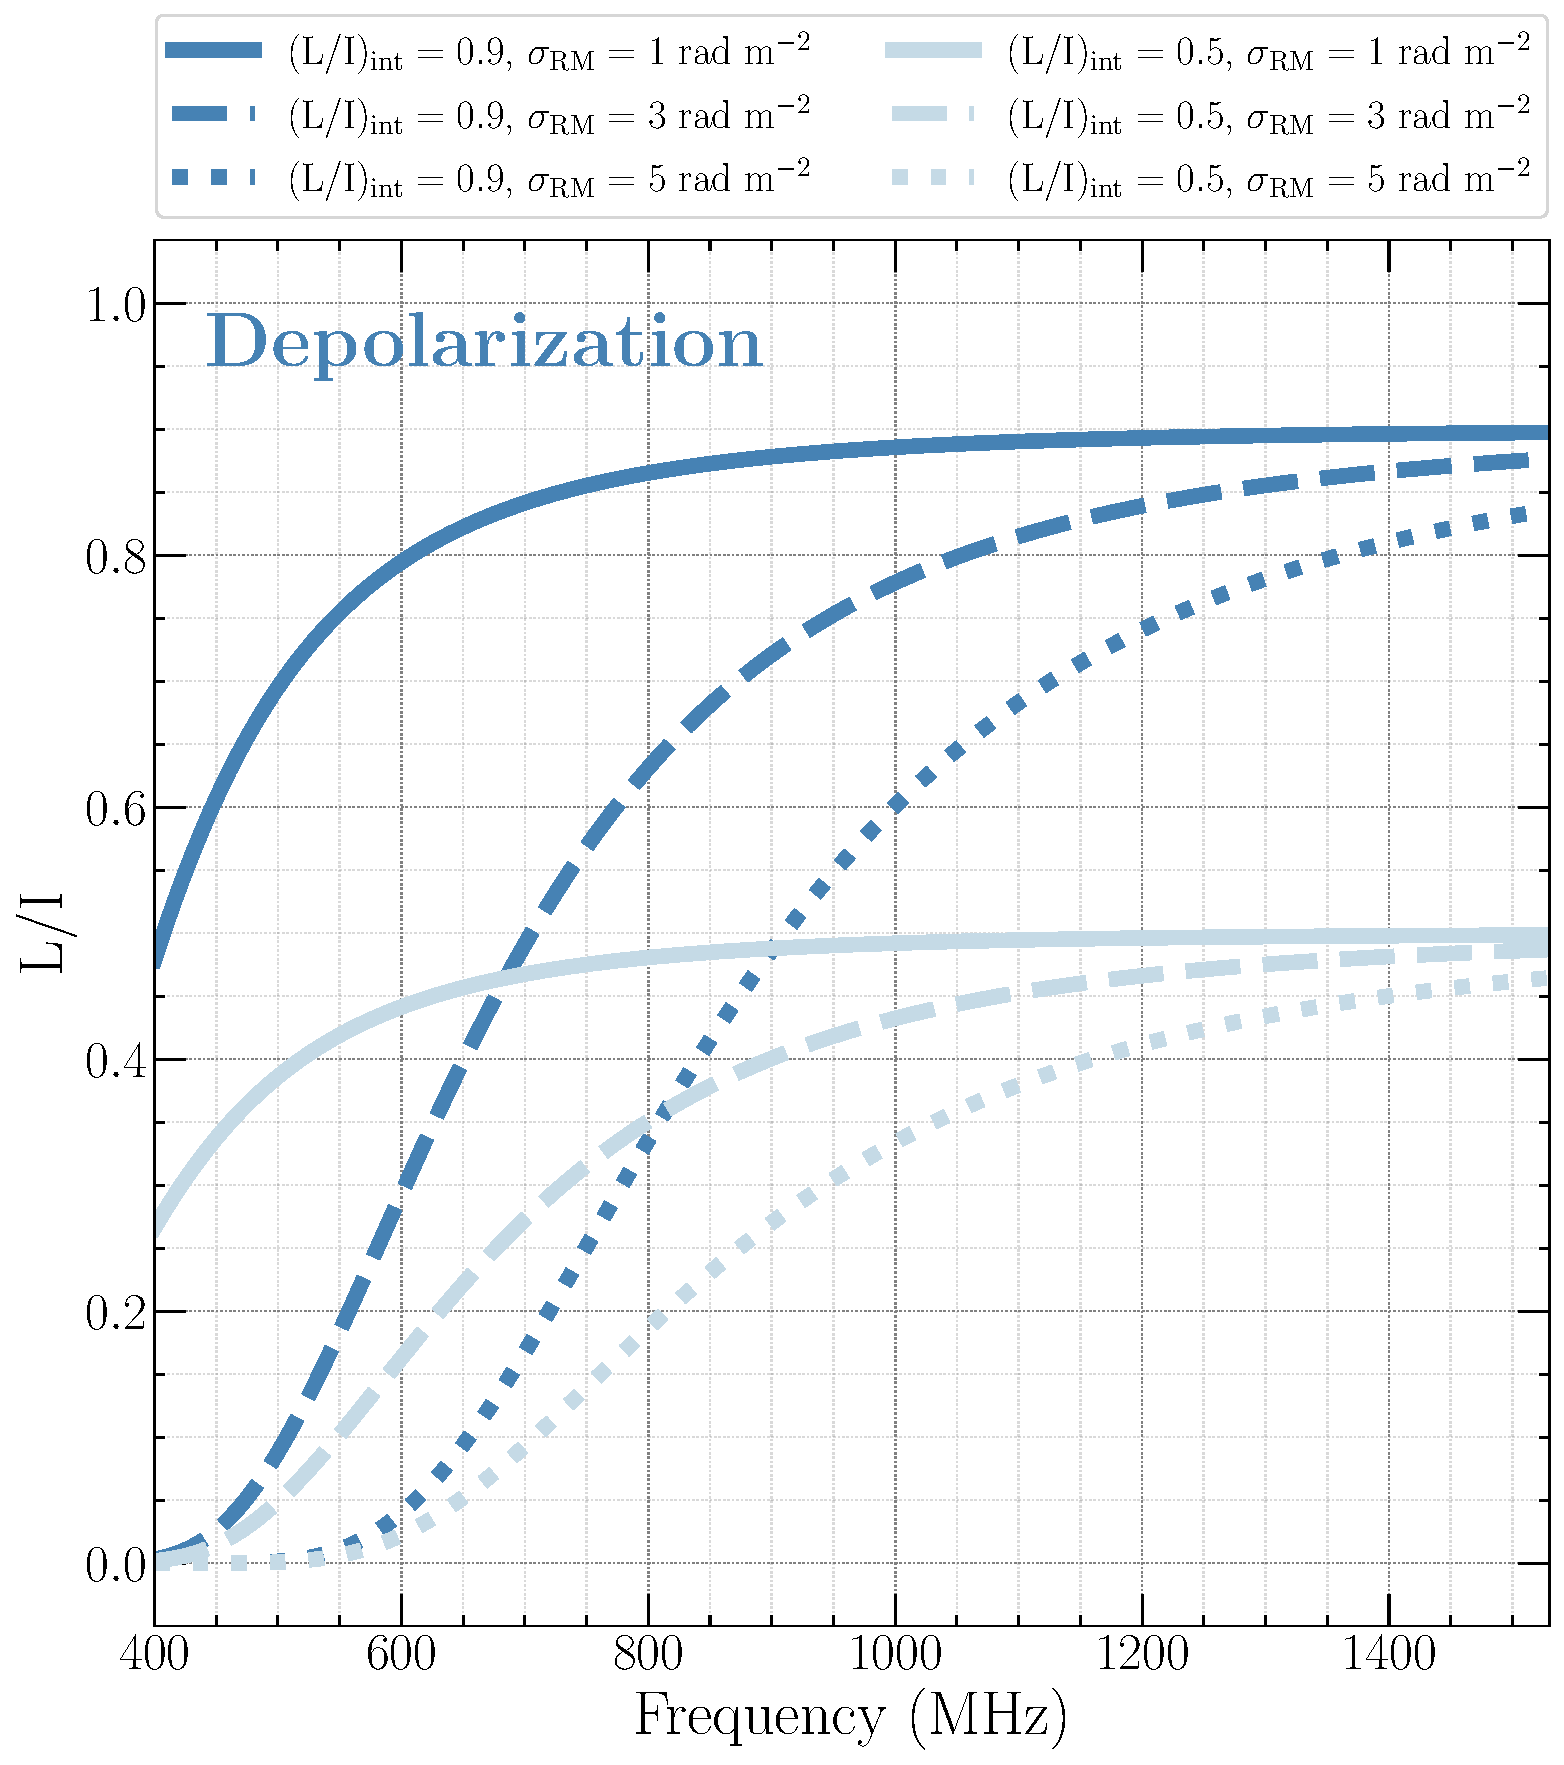
\includegraphics[width=0.329\textwidth]{model_2.pdf}
    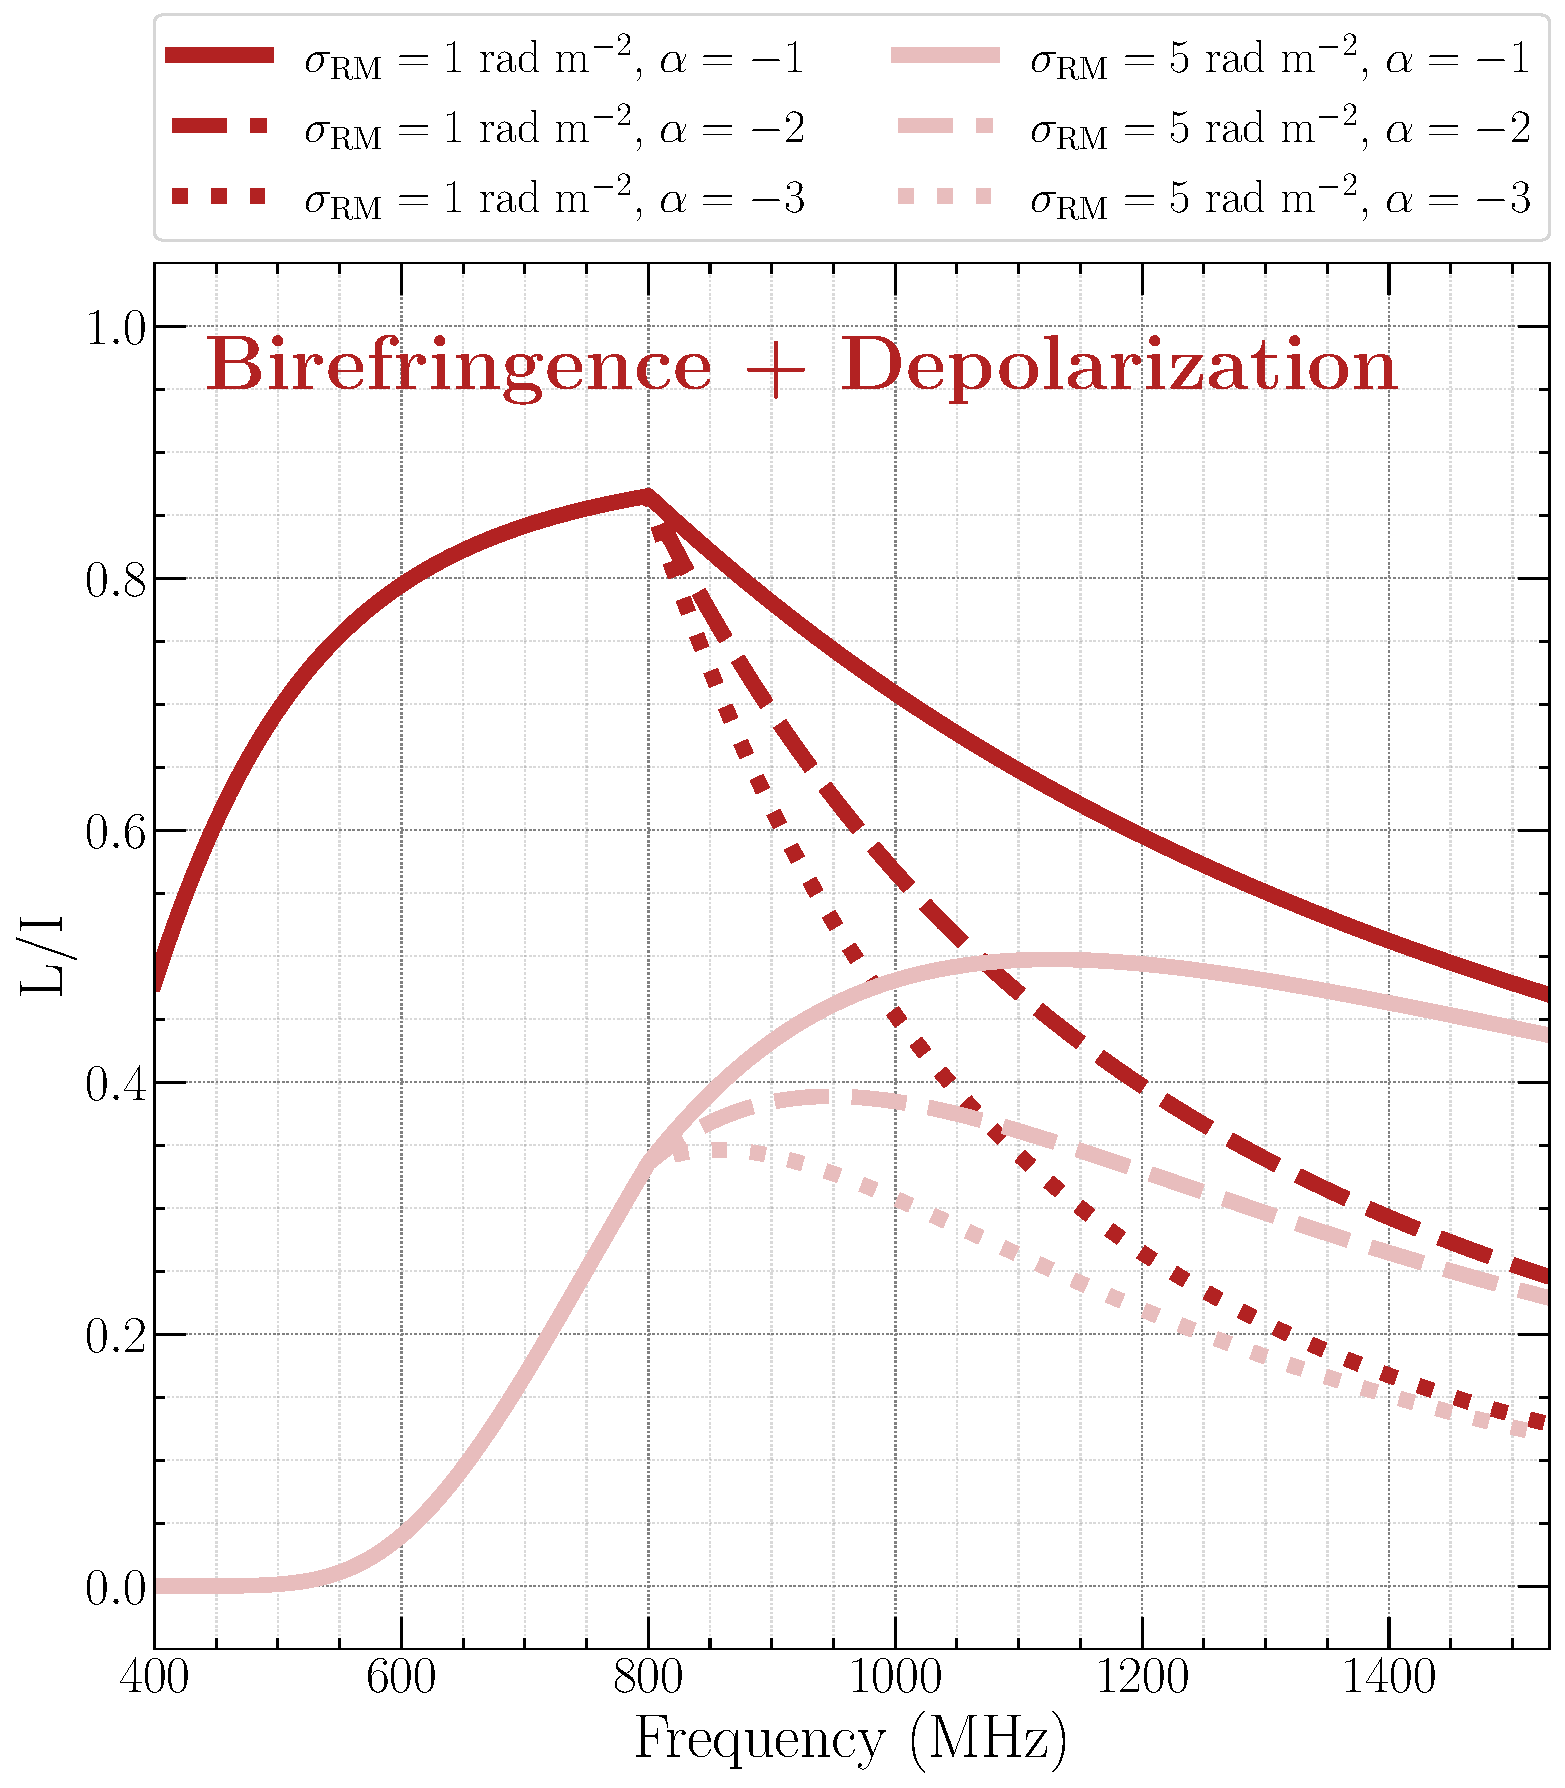
\includegraphics[width=0.329\textwidth]{model_3.pdf}
    \caption{(Left) Toy model of a constant $L/I$ versus frequency for different values of the intrinsic linear polarization fraction, $(L/I)_\mathrm{int}$. (Middle) Toy model of depolarization following Equation \ref{eq:model_2} for various input $\sigma_\mathrm{RM}$ values with $(L/I)_\mathrm{int}=0.9$ (dark lines) and $(L/I)_\mathrm{int}=0.5$ (faint lines). (Right) Toy model combining birefringence and depolarization effects (see Equation \ref{eq:model_3}). Dark lines show the model behavior for various $\alpha$ indices with $\sigma_\mathrm{RM} = 1~\mathrm{rad}~\mathrm{m}^{-2}$; faint lines show curves with $\sigma_\mathrm{RM} = 5~\mathrm{rad}~\mathrm{m}^{-2}$ and the same range of $\alpha$. All shown curves for the birefringence and depolarization model assume $(L/I)_\mathrm{int}=0.9$ and $\nu_c = 800$~MHz. The frequency range in all panels spans $400$~MHz (bottom of the CHIME/FRB band) to $1530$~MHz (top of the DSA-110 band).} 
    \label{fig:li_models}
\end{figure*}

\subsubsection{Model 1: Constant L/I} \label{subsec:model_1}
In the most straightforward model, the FRB is emitted at a constant intrinsic linear polarization fraction, $(L/I)_\mathrm{int}$, across its emitting bandwidth, and the signal is unaffected by any propagation effects. Then, the observed $L/I (\nu)$ is simply:
\begin{equation}
L/I (\nu) = (L/I)_\mathrm{int}\,. \label{eq:model_1}
\end{equation}
Examples of $L/I (\nu)$ following Equation \ref{eq:model_1} for a range of fiducial values are presented in the left panel of Figure \ref{fig:li_models}.

\subsubsection{Model 2: Depolarization} \label{subsec:model_2}
Decreasing $L/I (\nu)$ towards lower frequencies has been reported in a number of different radio sources, including in radio galaxies \citep[e.g.,][]{2012AJ....144..105H, 2014ApJS..212...15F}, pulsars \citep[e.g.,][]{2015A&A...576A..62N, 2019PASA...36...25X, 2021MNRAS.504..228S}, and FRBs \citep[e.g.,][]{2022Sci...375.1266F, 2025MNRAS.tmp.1894U, 2026ApJ..1000L..53P}, and it has been attributed to depolarization from intervening, inhomogeneous Faraday screens.

Consider now, that the FRB emitted with $(L/I)_\mathrm{int}$ passes through inhomogeneous plasma, causing the signal to be scattered to a finite angular size. It then undergoes differential Faraday rotation due to intervening spatial fluctuations in electron density and/or magnetic field strength. When the FRB is detected, these spatial RM variations are averaged across the observing beam, leading to a decrease in the observed linear polarization, $L/I (\nu)$, relative to $(L/I)_\mathrm{int}$ (referenced to zero wavelength):
\begin{equation}
L/I (\nu) = (L/I)_\mathrm{int}~\mathrm{exp} \left(-2 c^4 \nu^{-4} \sigma_\mathrm{RM}^2 \right)\,. \label{eq:model_2}
\end{equation}
Here, $c$ is the speed of light and $\sigma_\mathrm{RM}$ is a measure of the inhomogeneity in the magnetized scattering medium \citep{1966MNRAS.133...67B}. The middle panel of Figure \ref{fig:li_models} shows expected $L/I (\nu)$ spectra for a range of fiducial $\sigma_\mathrm{RM}$ and $(L/I)_\mathrm{int}$ values.

Equation \ref{eq:model_2} assumes a Gaussian distribution of RM fluctuations across the resolved source. Under other physical assumptions, e.g., if the RM structure function follows a power-law or if the RM fluctuations trace anisotropic turbulence, $L/I (\nu)$ may take on a power-law, or more complex, spectral shape \citep{1991MNRAS.250..726T, 2016ApJ...818..178L, 2016ApJ...825..154Z}. We choose to use the depolarization formulation described in Equation \ref{eq:model_2} as it has been adopted by previous FRB studies \citep[e.g.,][]{2022Sci...375.1266F, 2025MNRAS.tmp.1894U, 2026ApJ..1000L..53P}, allowing us to directly compare our results to the literature. However, understanding that this is a simplified case, we refrain from deriving physical properties of the depolarizing media (e.g., the distribution of $n_e$ and/or $B_\parallel$), and instead treat $\sigma_\mathrm{RM}$ as an analog for the level of inhomogeneity in local magnetoionic plasma that we can compare between FRB sources.

\subsubsection{Model 3: Birefringence and depolarization} \label{subsec:model_3}
Many complex polarization signatures, as a function of frequency and pulse phase, in coherent radio transients are thought to arise from propagation through birefringent plasma in a compact object magnetosphere, such as in pulsars \citep[e.g.,][]{1981A&A...100..107M, 1998MNRAS.301..235G, 2008MNRAS.388..261J, 2015A&A...576A..62N} and in long period radio transients \citep[e.g.,][]{2024MNRAS.535..909D, 2026arXiv260307857P}. One key spectral signature is decreasing linear polarization fraction with increasing frequency, which has been observed in many radio pulsar across several octaves in frequency. 

Radio emission from pulsars is thought to originate in the magnetosphere of the neutron star above their polar caps, with the emitting frequency relating to the height above the neutron star surface the emission is generated \citep[sometimes referred to as ``radius-to-frequency mapping'';][]{1975ApJ...196...51R}. Their polarized emission is thought to be comprised of two orthogonal propagation modes, the ordinary and extraordinary modes \citep{1975ApJ...196...83M}. The differing, frequency-dependent refractive indices of these two modes cause their beaming angles to diverge as they propagate through a birefringent medium, such as a neutron star magnetosphere \citep{1986ApJ...302..138B}. The angular separation between the two modes increases at lower frequencies (higher emission heights) where refraction is stronger such that the observer may only see emission from one of the two modes, which are each highly polarized. At higher frequencies (lower emission heights), the beaming angle between the two modes decreases and the observed emission becomes depolarized from the mixing of the orthogonal polarization modes. Empirically, \cite{1973ApJ...179L...7M} describe the $L/I (\nu)$ of these radio pulsars as a power-law decrease above a characteristic frequency, $\nu_c$, where the orthogonal modes become increasingly mixed, and the $L/I (\nu)$ is constant below $\nu_c$, when the observed emission is dominated by only one mode. 

If FRB emission is produced in the magnetosphere of a highly magnetized neutron star, it is plausible that the FRB spectra may have signatures of depolarization at both high (due to the birefringent magnetopsphere) and low (due to propagation through an inhomogeneous magnetoionic plasma in its local environment) frequencies. We combine these two effects in Model 3, such that the observed linear polarization fraction of the FRB emission is:
\begin{multline}
L/I (\nu) = ~\mathrm{exp} \left(-2 c^4 \nu^{-4} \sigma_\mathrm{RM}^2 \right)\\
\times
\begin{cases}
    (L/I)_\mathrm{int}, & \nu \leq \nu_c \\
    (L/I)_\mathrm{int} \left(\frac{\nu}{\nu_c}\right)^{\alpha}, & \nu > \nu_c 
\end{cases}
\,. \label{eq:model_3}
\end{multline}
Example $L/I (\nu)$ spectra for fiducial values of $(L/I)_\mathrm{int}$, $\nu_c$, $\sigma_\mathrm{RM}$, and $\alpha$ are plotted in the rightmost panel of Figure \ref{fig:li_models}.

\subsection{Polarization angle} \label{sec:models_pa}
From the derotated Stokes $Q$ and $U$ dynamic spectra (denoted by the subscript ``derot'' for clarity) we can derive the observed PA as a function of time, $t$, across the burst envelope as:
\begin{equation}
\mathrm{PA}(t) = \frac{1}{2} \mathrm{arctan} \left( \frac{U_\mathrm{derot}(t)}{Q_\mathrm{derot}(t)} \right)\,. \label{eq:pa}
\end{equation}
PA uncertainties are calculated by propagating uncertainties in the $Q_\mathrm{derot}$ and $U_\mathrm{derot}$ spectra, following the procedure detailed by \cite{2019ApJ...878...92V}. We mask out any points in the PA profile below a linearly-polarized $\mathrm{S/N} < 5$, a conservative threshold above which the PA uncertainties have been shown to be robust \citep[see Appendix B by][]{2024ApJ...968...50P}. Since the CHIME/FRB polarization pipeline does not calibrate for an absolute PA due to unknown beam phase effects off of CHIME's meridian axis, we focus our analysis on the relative PA evolution across the burst. Hence, we center both the $400-800$~MHz and $1280-1530$~MHz PA profiles to have a median of $0^\circ$. Following the procedure described by \cite{2024ApJ...968...50P}, we quantify the magnitude of PA variability in a given PA$(t)$ timeseries by evaluating the goodness of fit between the observed PA profile, centered at $0^\circ$, and a constant PA$(t) = 0^\circ$ model using a reduced $\chi_\nu^2$ test. We use a threshold of $\chi_\nu^2 \geq 5$, above which we consider the PA profile to be variable.

Given our large effective bandwidth for these codetected FRBs, we aim to characterize whether PA profiles of scattered FRBs become flattened at low frequencies due to mixing of signal from different pulse phases in the scattering tail. In the FRB literature, this effect is most clearly seen in FRB~20250316A, in which a clear PA swing of $30^\circ$ at $\sim800$~MHz becomes suppressed by scatter broadening at $\sim 400$~MHz, where the PA is almost entirely constant across the burst envelope \citep[see Figure 5 by][]{2025ApJ...989L..48C}. We search for such signals in our codetected FRBs by applying the following criteria: (i) $\chi_\nu^2 \geq 5$ at $1280-1530$~MHz while $\chi_\nu^2 < 5$ at $400-800$~MHz, (ii) the amplitude of the maximum PA variation across the profile decreases from $1280-1530$ to $400-800$~MHz and (iii) there is a clear coherent PA swing at $1280-1530$~MHz. The latter criterion ensures that the large $\chi_\nu^2$ is not dominated by, e.g., PA variation between subcomponents, each of which may have constant PA profiles. In cases where the FRB is sufficiently bright at $400-800$~MHz, we further subband the data to compute PA profiles at $400-600$~MHz and $600-800$~MHz, respectively.

\section{Results} \label{sec:results}
\subsection{FRB magnetoionic environments} \label{sec:results_host_env}
The observed RMs are summarized along with subsequent results in Table \ref{tb:host_props}. Performing RM-synthesis on joint CHIME/FRB$-$DSA-110 spectra only marginally improves the theoretical RM uncertainty while causing significant artifacts in the FDF due to differences in the relative polarized intensity scalings between instruments, and irregular frequency sampling. Thus, we opt to report the observed RM, $\mathrm{RM}_\mathrm{obs}$, from the CHIME/FRB data as the lower frequency and larger bandwidth observations provide greater accuracy in the RM determination; we confirm that the FDF peaks of the CHIME/FRB and DSA-110 data agree to within their respective full-width-half-maximum for each codetected FRB. Polarization properties of these FRBs will also be provided in future catalogs by the CHIME/FRB and DSA-110 teams, respectively (M.~Ng et al.~in prep.; F.~Verdi et al.~in prep.). The observed DM, $\mathrm{DM}_\mathrm{obs}$, and host galaxy redshift, $z$, of these FRBs are reported in paper I and adopted for this work. 

$\mathrm{DM}_\mathrm{obs}$ and $\mathrm{RM}_\mathrm{obs}$ can be written as the sum of individual contributions from plasma along the LOS:
\begin{multline}
\mathrm{DM}_\mathrm{obs} = \mathrm{DM}_{\mathrm{ion}} + \mathrm{DM}_{\mathrm{disk}} + \mathrm{DM}_{\mathrm{halo}} + \mathrm{DM}_{\mathrm{IGM}}(z) \\
+ \frac{\mathrm{DM}_{\mathrm{host}}}{(1 + z)}~\mathrm{pc}~\mathrm{cm}^{-3}\,; \label{eq:dm_comps}
\end{multline}
\begin{multline}
\mathrm{RM}_\mathrm{obs} = \mathrm{RM}_{\mathrm{ion}} + \mathrm{RM}_{\mathrm{disk}} + \mathrm{RM}_{\mathrm{halo}} + \mathrm{RM}_{\mathrm{IGM}}(z) \\
+ \frac{\mathrm{RM}_{\mathrm{host}}}{(1+z)^2}~\mathrm{rad}~\mathrm{m}^{-2}\,, \label{eq:rm_comps}
\end{multline}
where ``ion" refers to the Earth's ionosphere, ``disk" and ``halo", are the Milky Way disk and halo, respectively, ``IGM" is the intergalactic medium and ``host" is the host galaxy. We can calculate the electron density-weighted average LOS magnetic field strength in the FRB host galaxy using the $\mathrm{DM}_{\mathrm{host}}$ and $\mathrm{RM}_{\mathrm{host}}$:
\begin{equation}
\left<B_{\parallel,\mathrm{host}}\right> = 1.232 \frac{\mathrm{RM}_\mathrm{host}}{\mathrm{DM}_\mathrm{host}}~\mu\text{G}\,. \label{eq:b_host}
\end{equation}

We employ Monte Carlo random sampling to determine $\mathrm{DM}_\mathrm{host}$, $\mathrm{RM}_\mathrm{host}$, and $\left<B_{\parallel,\mathrm{host}}\right>$, following the procedure described by \cite{2025ApJ...982..146P}. For each FRB, we perform 10$^4$ trials, drawing foreground DM and RM contributions from assumed distributions and using the host galaxy redshift to convert to rest-frame quantities. The median of the resulting $\mathrm{DM}_\mathrm{host}$, $\mathrm{RM}_\mathrm{host}$, and $\left<B_{\parallel,\mathrm{host}}\right>$ distributions are taken as the maximum likelihood estimates with 68\% confidence intervals representing the associated uncertainties. $\mathrm{DM}_\mathrm{obs}$ and $\mathrm{RM}_\mathrm{obs}$ are drawn from Gaussian distributions centered on their measured values and with standard deviation equal to their uncertainties. We assume that the ionospheric contribution is negligible \citep[typically $\mathrm{DM}_\mathrm{ion} \lesssim 10^{-5}~\mathrm{pc}~\mathrm{cm}^{-3}$ and $\mathrm{RM}_\mathrm{ion} \lesssim 1~\mathrm{rad}~\mathrm{m}^{-2}$;][]{2016ApJ...821...66L, 2019MNRAS.484.3646S}. $\mathrm{DM}_{\mathrm{disk}}$ is drawn from a Gaussian with mean equal to the DM estimated by the NE2025 model towards the FRB position \citep{2026arXiv260211838O} and assuming a uniform $20$\% uncertainty. $\mathrm{DM}_\mathrm{halo}$ is drawn from a Lognormal distribution with mean $\mathrm{log}_{10}(30~\mathrm{pc}~\mathrm{cm}^{-3})$ and a 0.2~dex standard deviation \citep{2015MNRAS.451.4277D,2020ApJ...888..105Y,2023ApJ...946...58C}. $\mathrm{RM}_{\mathrm{disk}} + \mathrm{RM}_{\mathrm{halo}}$ follow a Gaussian distribution based on the reconstructed Galactic mean RM and variance at the FRB position \citep{2022A&A...657A..43H}. $\mathrm{DM}_\mathrm{IGM}$ is sampled from the probability distribution function presented in Equation 1 of \cite{2024ApJ...965...57B}, based on the empirical $\mathrm{DM}_\mathrm{IGM} - z$ relation. $\mathrm{RM}_\mathrm{IGM}$ follows a Gaussian distribution centered at $0~\mathrm{rad}~\mathrm{m}^{-2}$ with standard deviation $6~\mathrm{rad}~\mathrm{m}^{-2}$ \citep{2010MNRAS.409L..99S}. The best-fit $\mathrm{DM}_\mathrm{host}$, $\mathrm{RM}_\mathrm{host}$, and $\left<B_{\parallel,\mathrm{host}}\right>$ for each codetected FRB associated with a host galaxy that has a measured spectroscopic redshift is presented in Table \ref{tb:host_props}.

\setlength{\tabcolsep}{0.08pt}
\setlength\extrarowheight{2pt}
\setlength{\LTcapwidth}{1.0\textwidth}
\begin{table}[ht!]
\begin{center}
\caption{Summary of magnetoionic properties for the 12 codetected FRB host environments.} \label{tb:host_props}
\begin{tabular}{ccccc}
\hline
\hline
TNS Name & $\mathrm{RM}_\mathrm{obs}$ & $\mathrm{RM}_\mathrm{host}$ & $\mathrm{DM}_\mathrm{host}$ & $\left<B_{\parallel,\mathrm{host}}\right>$\\
 & (rad m$^{-2}$) & (rad m$^{-2}$) & (pc cm$^{-3}$) & ($\mu$G)\\
\hline
FRB~20220207C & $-161.54(1)$ & $-170^{+20}_{-19}$ & $141^{+18}_{-27}$ & $-1.5^{+0.2}_{-0.4}$\\
FRB~20220310F & $-5.3(2)$ & $+19^{+21}_{-21}$ & $136^{+69}_{-81}$ & $+0.18^{+0.36}_{-0.19}$\\
FRB~20220506D & $+32(4)\tablenotemark{a}$ & $+70^{+27}_{-28}$ & $133^{+50}_{-70}$ & $+0.67^{+0.73}_{-0.30}$\\
FRB~20221113A & $-13.65(9)$ & $+50^{+30}_{-30}$ & $172^{+48}_{-76}$ & $+0.38^{+0.37}_{-0.23}$\\
FRB~20221203A$\tablenotemark{b}$ & $+21.0(2)$ & $-$ & $-$ & $-$\\
FRB~20230307A & $-473.49(9)$ & $-756^{+15}_{-15}$ & $464^{+56}_{-130}$ & $-2.0^{+0.2}_{-0.8}$\\
FRB~20230325A$\tablenotemark{b}$ & $-10.48(2)$ & $-$ & $-$  & $-$\\
FRB~20230814B & $+23.3(1)$ & $+39^{+45}_{-46}$ & $309^{+103}_{-161}$ & $+0.2^{+0.3}_{-0.2}$\\
FRB~20230913A & $-81.39(3)$ & $-164^{+27}_{-25}$ & $285^{+59}_{-111}$ & $-0.72^{+0.17}_{-0.45}$\\
FRB~20240122A$\tablenotemark{b}$ & $-2.4(3)$ & $-$ & $-$ & $-$\\
FRB~20240203A & $+178.18(9)$ & $+221^{+19}_{-19}$ & $135^{+22}_{-35}$ & $+2.0^{+0.7}_{-0.3}$\\
FRB~20240229A & $-11.21(1)$ & $+3^{+13}_{-13}$ & $305^{+57}_{-113}$ & $+0.01^{+0.06}_{-0.06}$\\
\hline
\hline
\end{tabular}
\end{center}
\tablenotetext{$a$}{Obtained from DSA-110 data as the linearly polarized intensity of the CHIME/FRB detection was too low to robustly measure RM.}
\tablenotetext{$b$}{Does not have an associated host galaxy with a measured spectroscopic redshift.}
\end{table}


\subsection{Linear polarization} \label{sec:results_li}
We utilize an ensemble Markov Chain Monte Carlo (MCMC) sampling routine, implemented with the {\tt emcee} package \citep{2013PASP..125..306F}, to fit the observed $L/I$ spectra of each codetected FRB to the three models presented in Section \ref{sec:models_li} (Equations \ref{eq:model_1}$-$\ref{eq:model_3}). Assuming Gaussian uncertainties, the log-likelihood is defined as:
\begin{multline}
\mathrm{ln}~\mathcal{L} = -\frac{1}{2}\sum_i \bigg[ \left( \frac{(L/I)_i - (L/I)_{\mathrm{model,}i}}{\sigma_{(L/I),i}} \right)^2 \\
+ \mathrm{ln} \left(2 \pi \sigma_{(L/I),i}^2 \right) \bigg], \label{eq:log_likelihood}
\end{multline}
where $(L/I)_i$ is the observed linear polarization fraction and $\sigma_{(L/I),i}$ is the associated measurement uncertainty; $(L/I)_{\mathrm{model,}i}$ is the expected model $L/I$ following one of Equations \ref{eq:model_1}, \ref{eq:model_2}, or \ref{eq:model_3}. We adopt uniform priors over the following ranges: $0 \leq(L/I)_\mathrm{int} \leq 1$, $0~\mathrm{rad}~\mathrm{m}^{-2} \leq \sigma_\mathrm{RM} \leq 100~\mathrm{rad}~\mathrm{m}^{-2}$, $0~\mathrm{MHz} < \nu_c <10^4~\mathrm{MHz}$, and $-10 < \alpha < 0$. Maximum-likelihood estimates for each parameter are determined as the medians of the resulting posterior distributions, with uncertainties quoted as the 16$^\mathrm{th}$ and 84$^\mathrm{th}$ percentiles. We conduct model comparison in two steps: (i) we compute the Bayesian Information Criterion \citep[BIC;][]{1978AnSta...6..461S} and determine which model minimizes the BIC for a given FRB $L/I$ spectra, and (ii) if the BIC between two or more models are similar (to within $\lesssim 1\%$) and their model spectra are visually similar, we default to the simplest (i.e., with the least physical assumptions) model. 

For each codetected FRB, we plot the observed $L/I$ spectra and the MCMC model fits for our three $L/I(\nu)$ models in Figure \ref{fig:li_spectra}. The best-fit $L/I$ model is identified in the bottom right of each panel and the maximum-likelihood estimates for those model parameters are provided in Table \ref{tb:model_params}. Note that the lowest frequency bin for both FRBs~20220506D and 20221203A are upper limits in $L/I$ but, for the purposes of our model fitting, they are treated as data points. This is specifically because each of the upper limits show a large downturn in $L/I$ from the next-highest frequency bin. By treating the upper limit as a measured $L/I$, we are effectively able to constrain an upper limit on $\sigma_\mathrm{RM}$ in these two cases rather than make a direct measurement (this caveat is also reflected in Table \ref{tb:model_params}). For the FRBs best fit by Equation \ref{eq:model_3}, $\nu_c$ has large uncertainties as it falls in the observing-frequency gap between the top of the CHIME/FRB and bottom of the DSA-110 bands ($800-1280$~MHz).

Overall, we find that $4/12$ FRBs favor the constant $L/I$ model, $5/12$ prefer the depolarization model, and $3/12$ are best described by the combination of magnetospheric birefringence effects and beam depolarization. Two of the three FRBs in the latter category (FRBs~20230307A and 20240229A) show a clear downtick in $L/I$ towards $400$~MHz, while the $L/I$ of FRB~20230913A increases from DSA-110 to CHIME/FRB frequencies, and it remains approximately constant across $400-800$~MHz. Thus, significant depolarization is observed in $7/12$ FRBs in our sample.

\begin{figure*}
    \centering \hspace{14pt}
    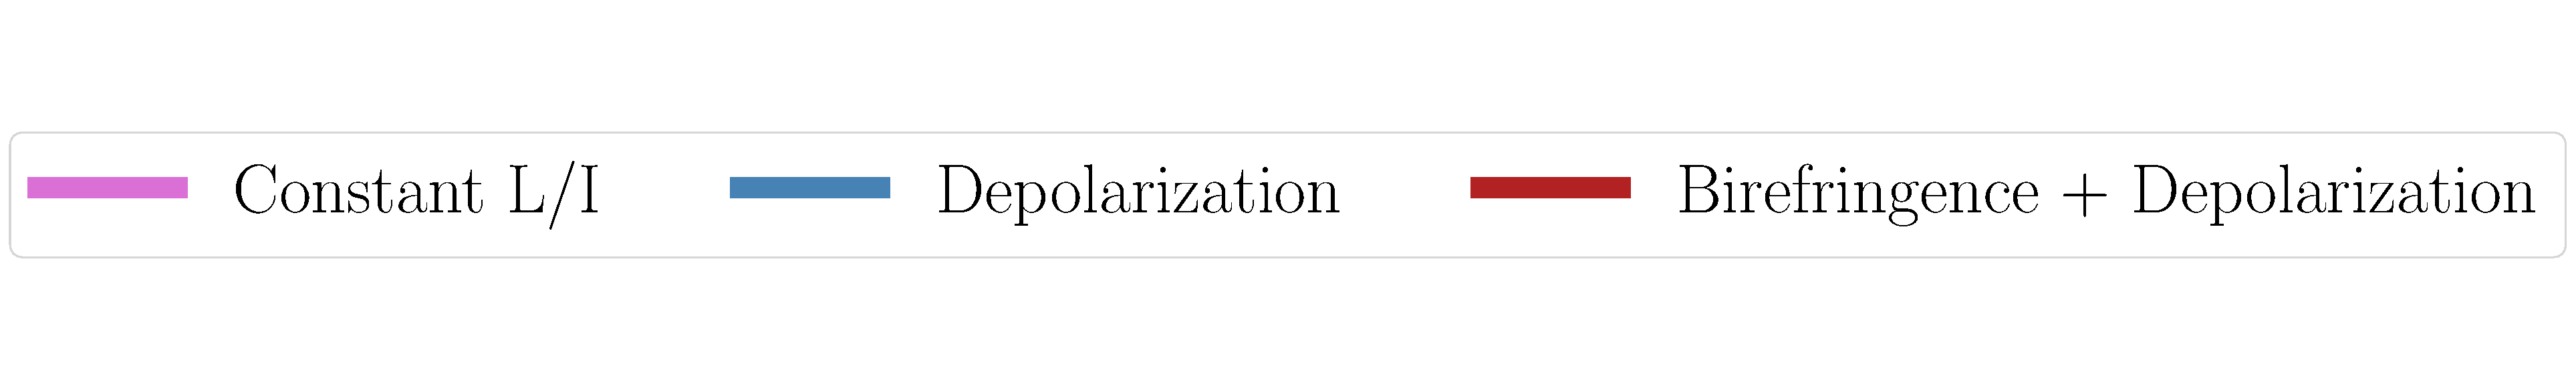
\includegraphics[width=0.82\textwidth]{legend_lispectra.pdf}\\ \vspace{-20pt}
    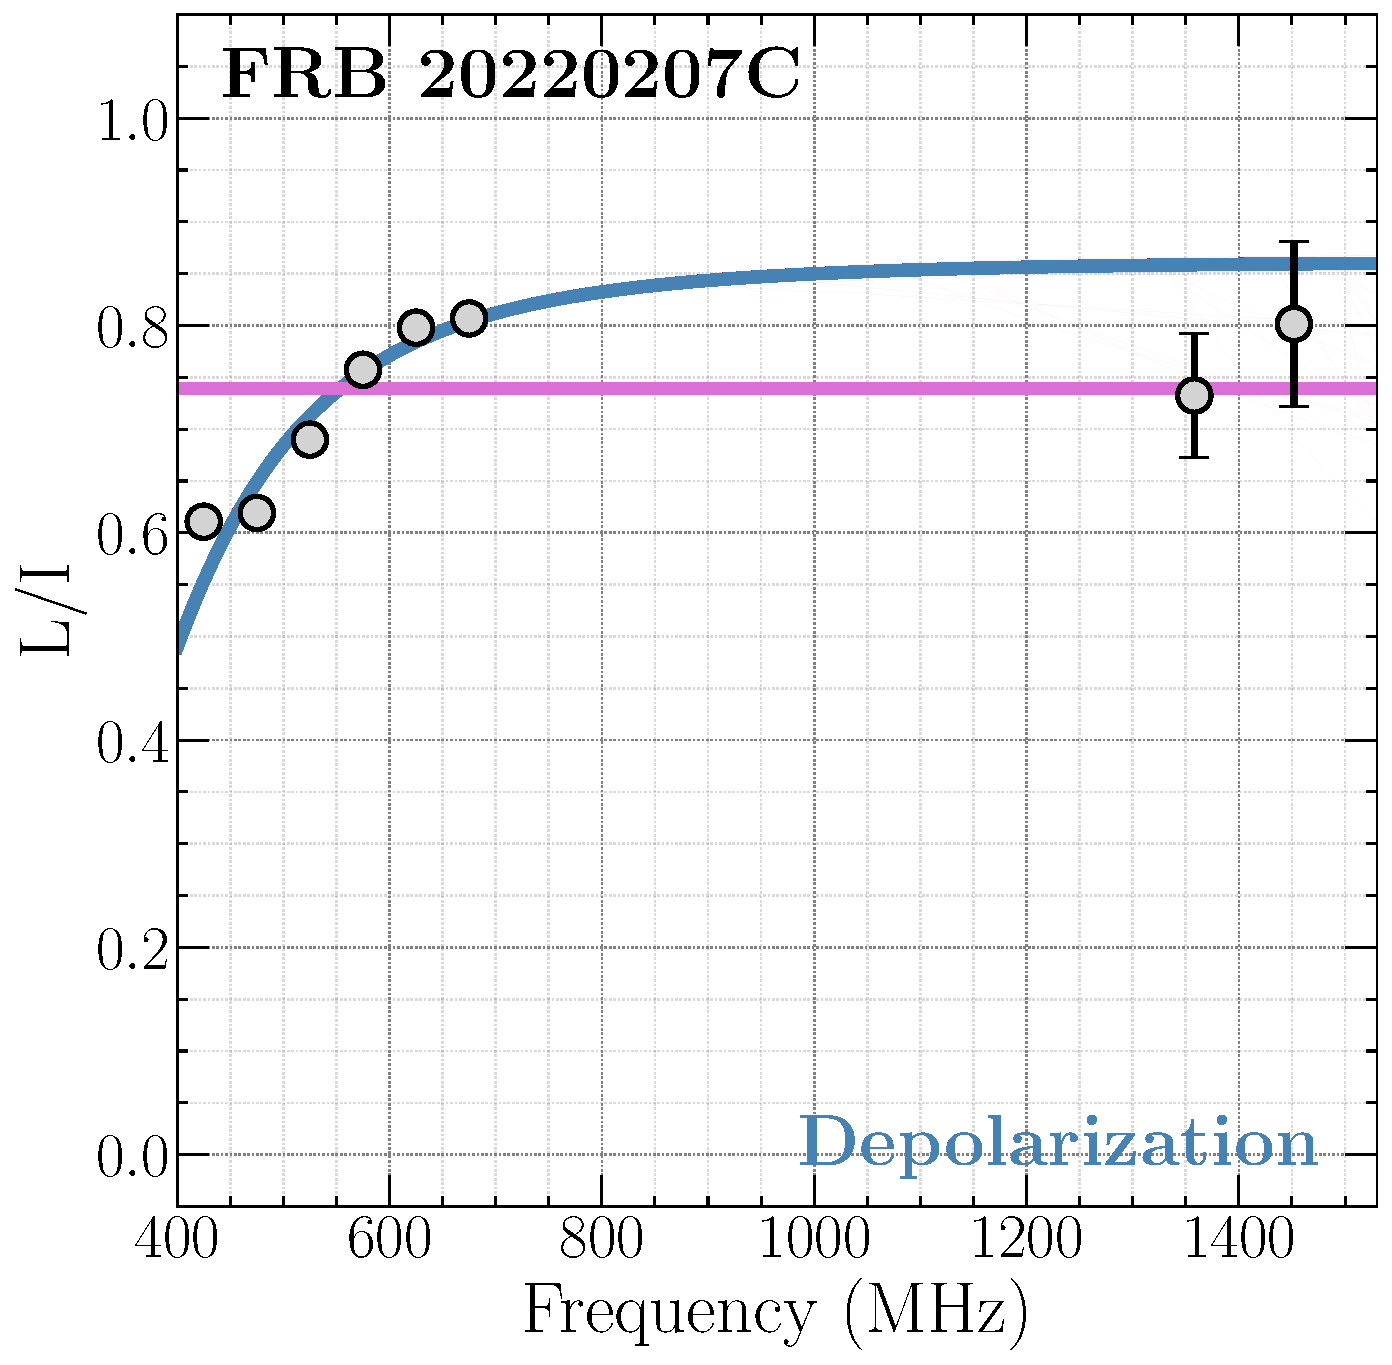
\includegraphics[width=0.28\textwidth]{frb_20220207c_lispectra.pdf}
    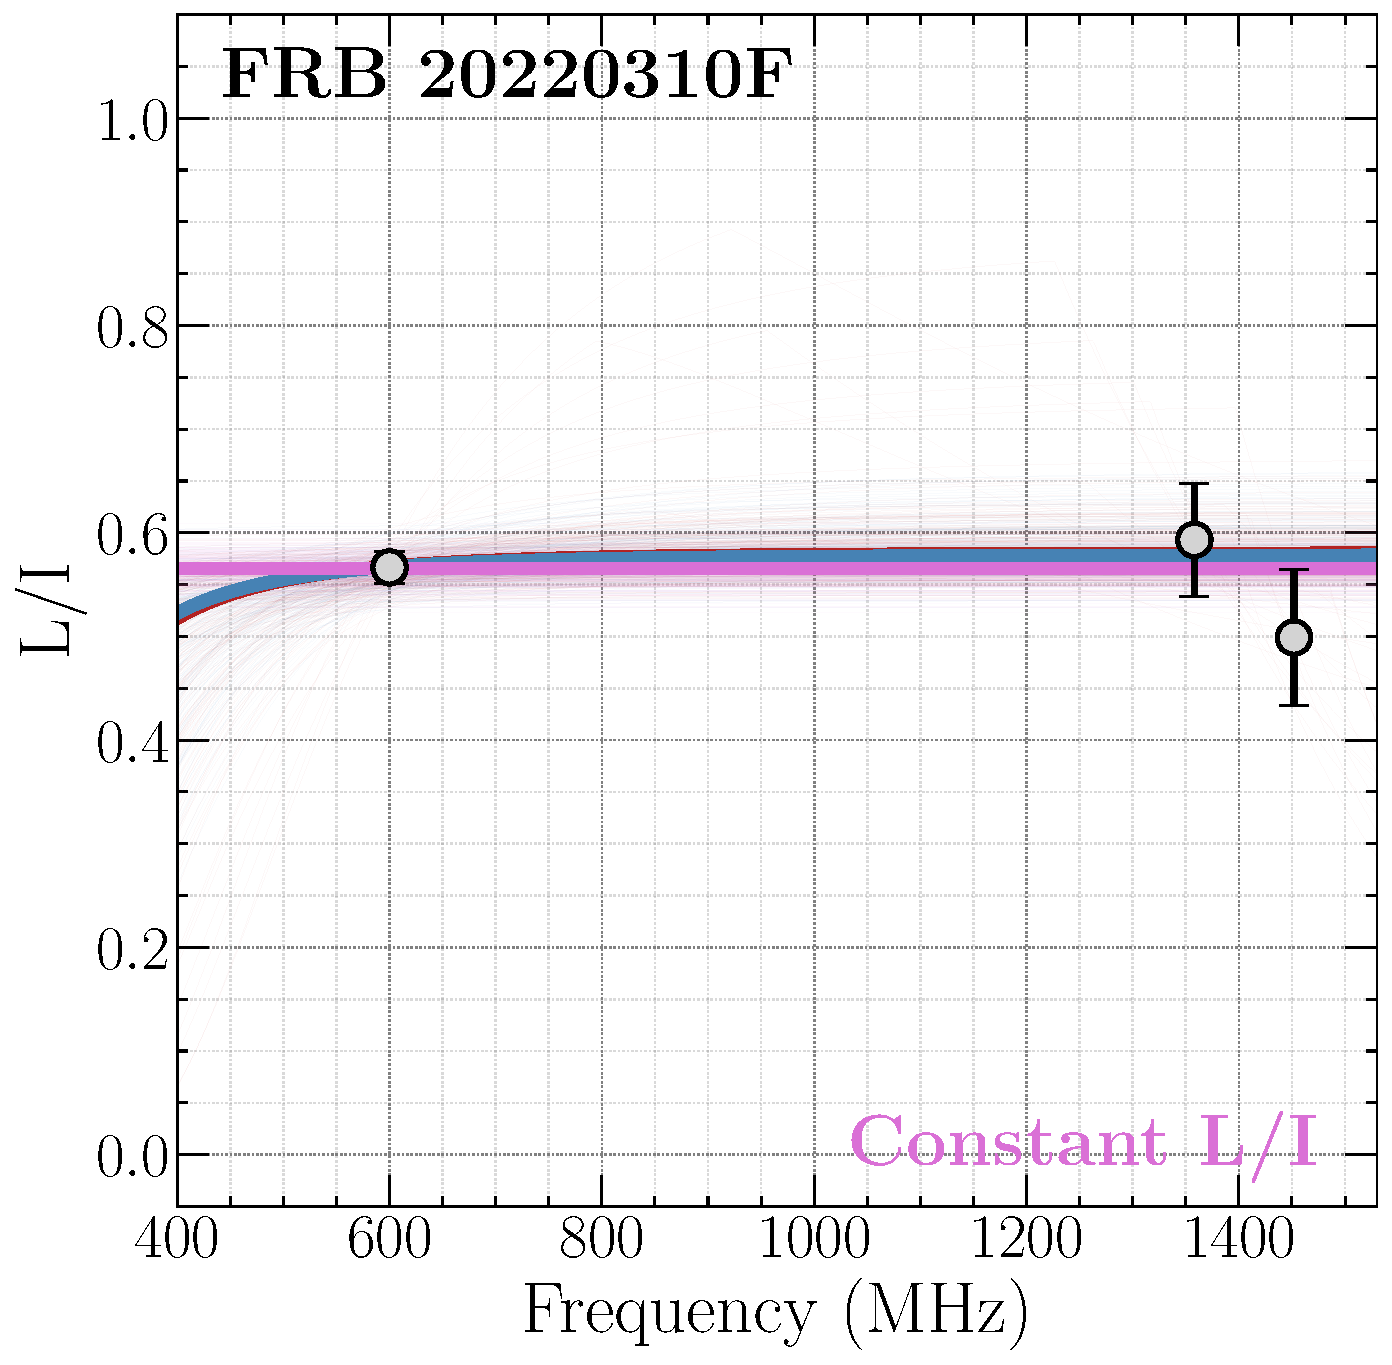
\includegraphics[width=0.28\textwidth]{frb_20220310f_lispectra.pdf}
    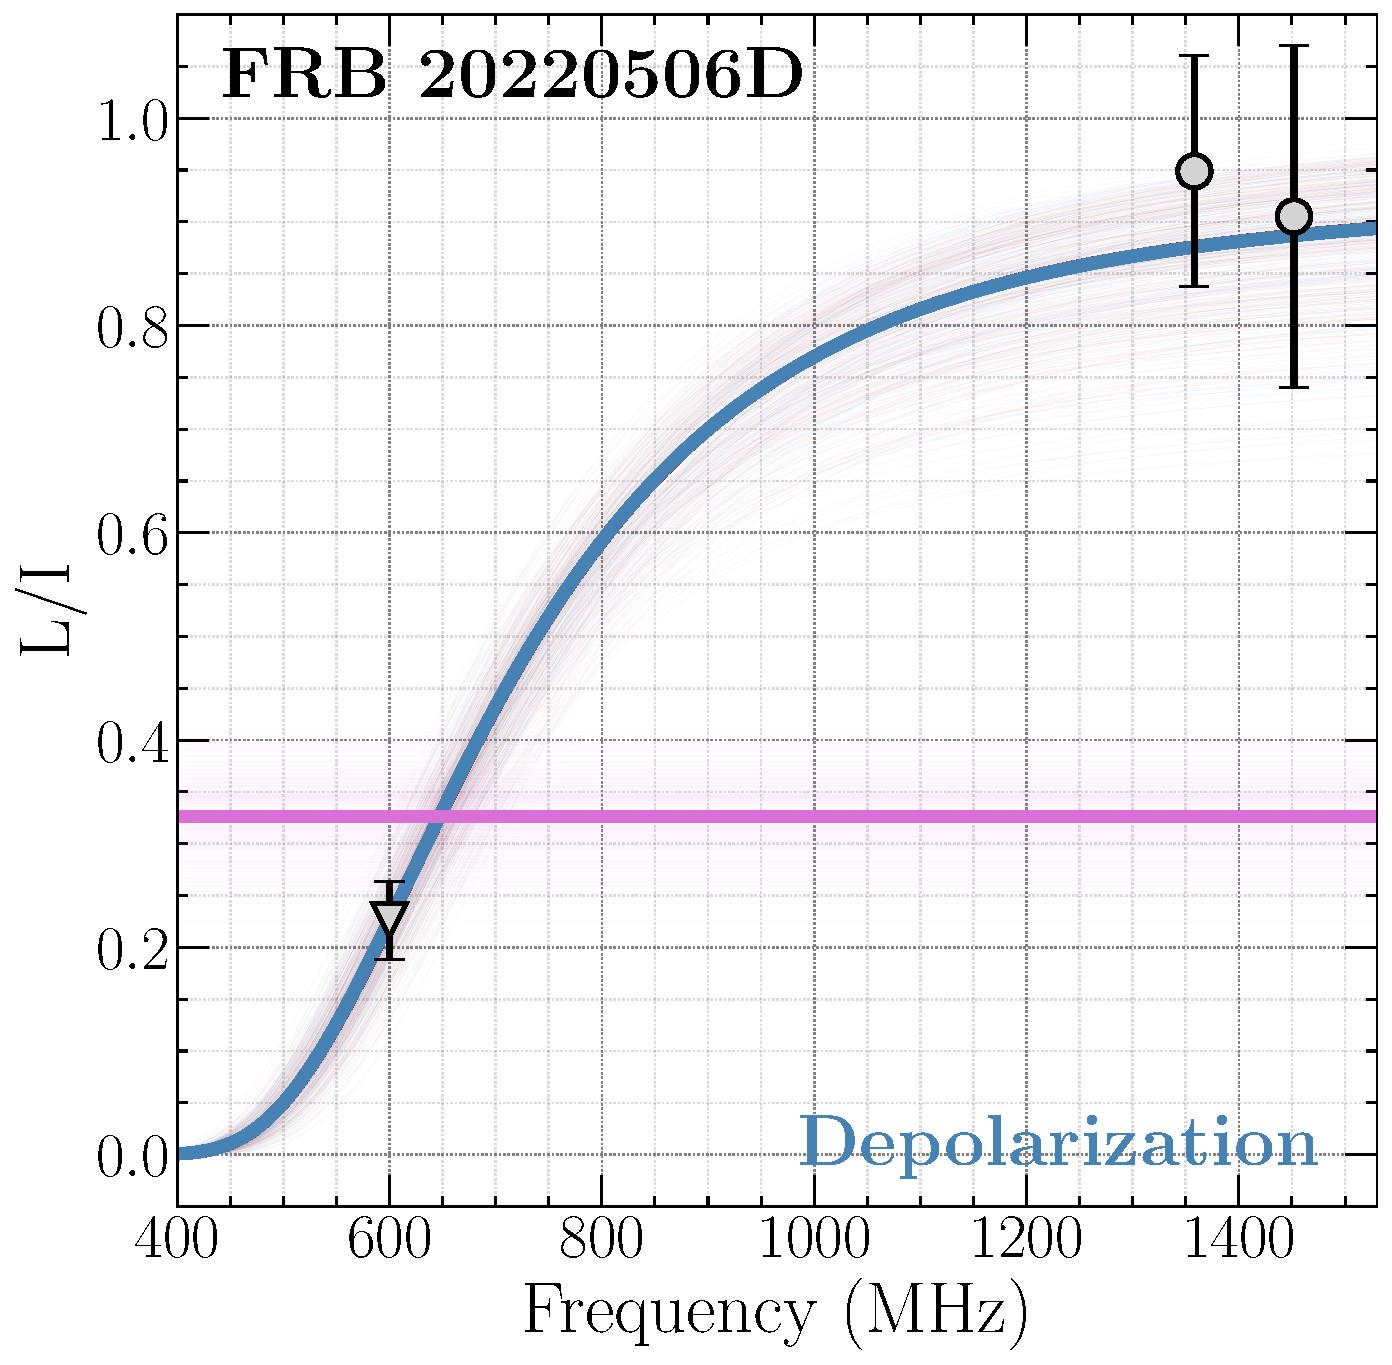
\includegraphics[width=0.28\textwidth]{frb_20220506d_lispectra.pdf}
    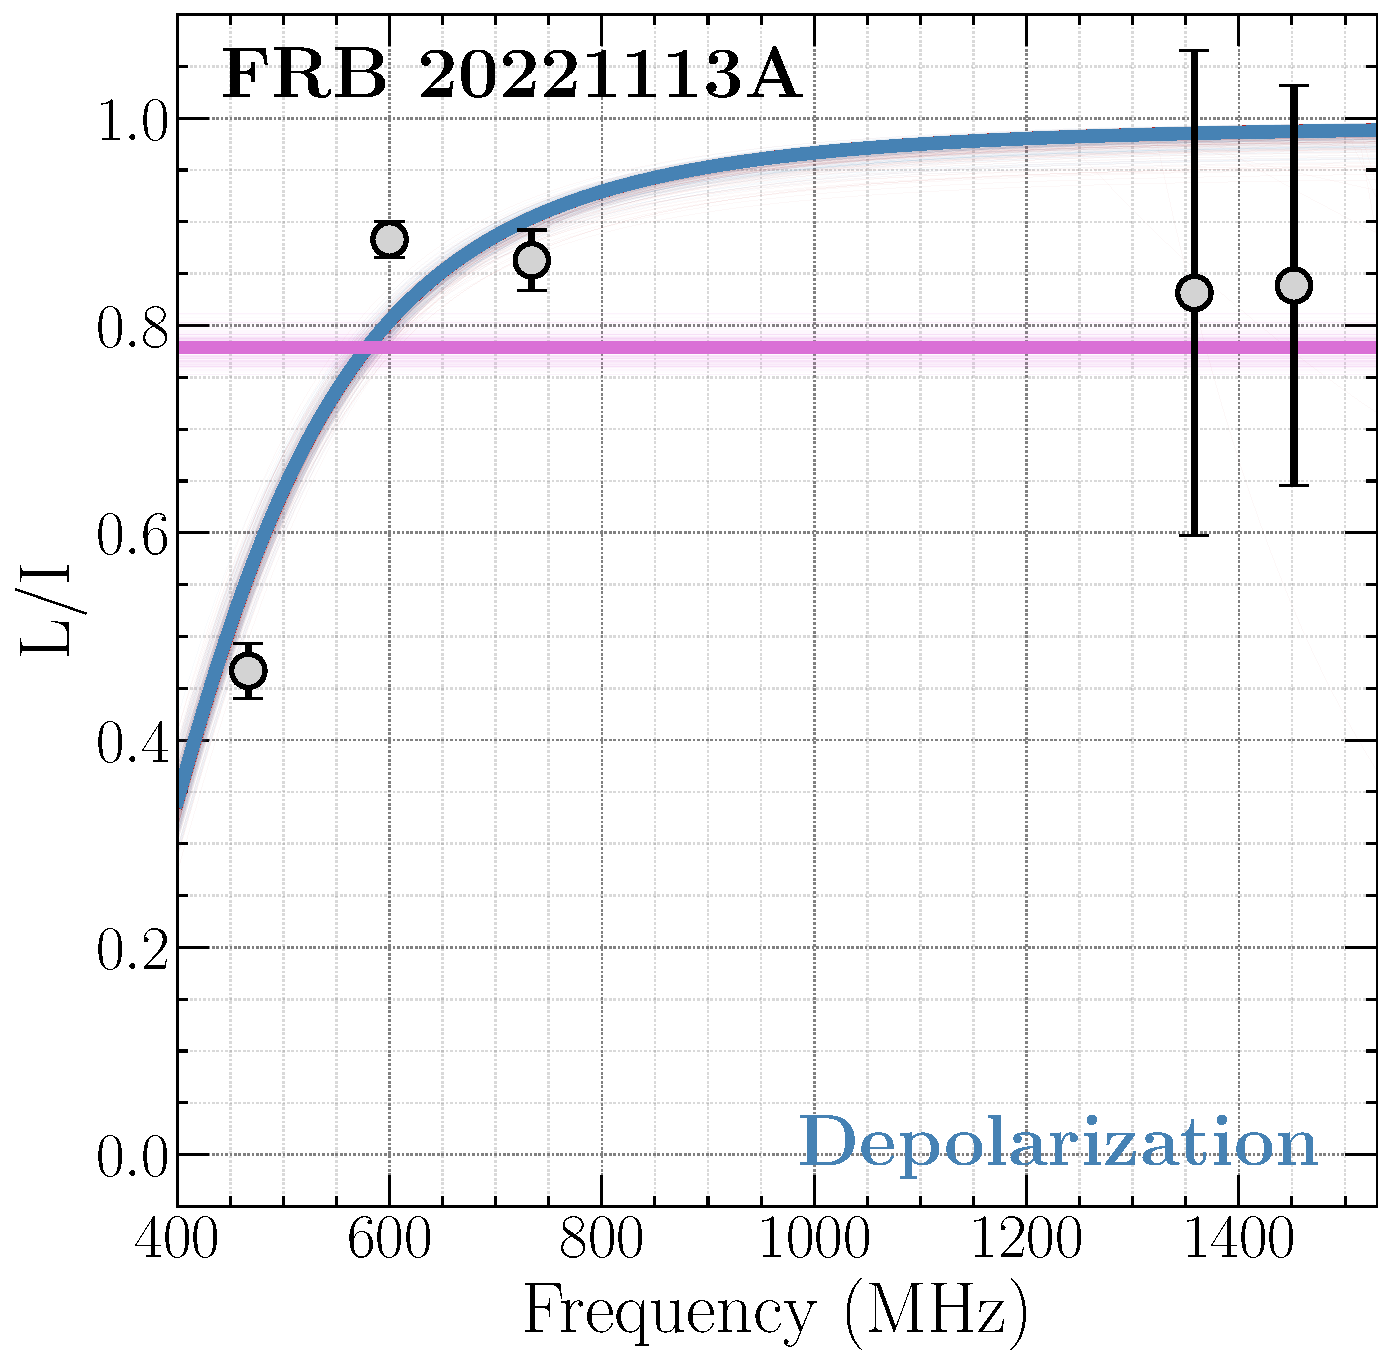
\includegraphics[width=0.28\textwidth]{frb_20221113a_lispectra.pdf}
    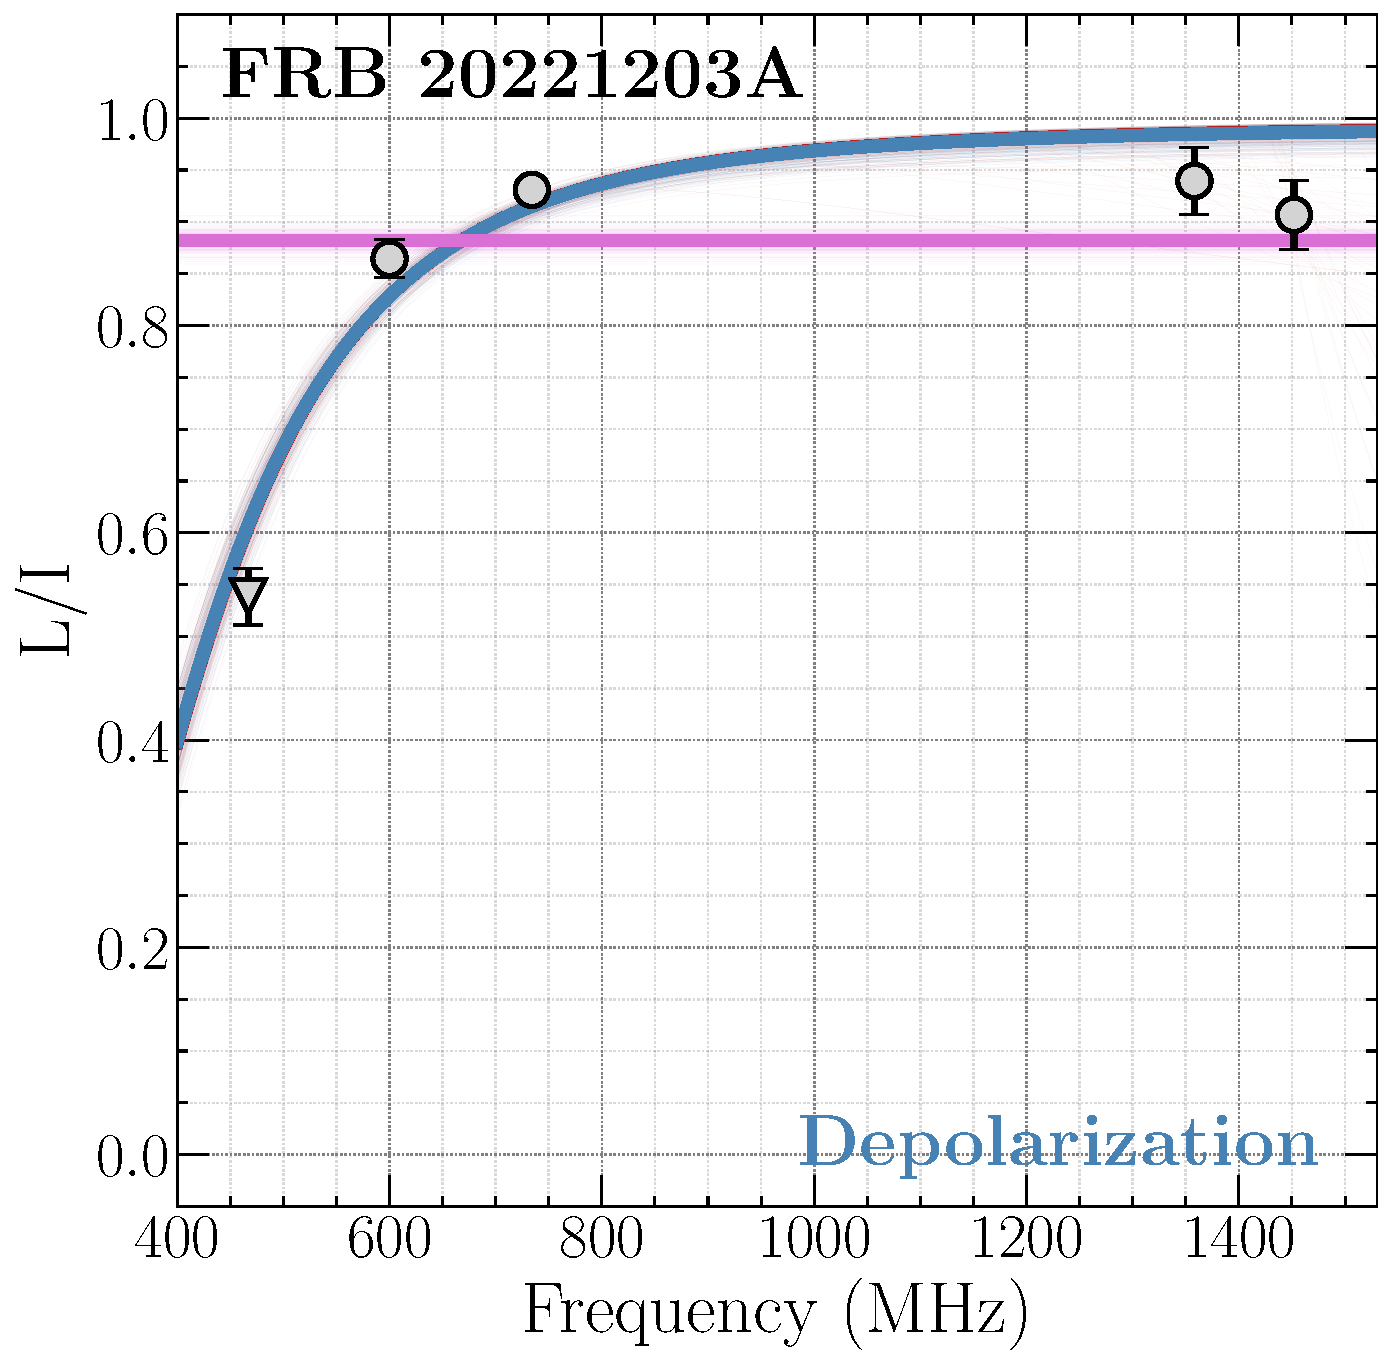
\includegraphics[width=0.28\textwidth]{frb_20221203a_lispectra.pdf}
    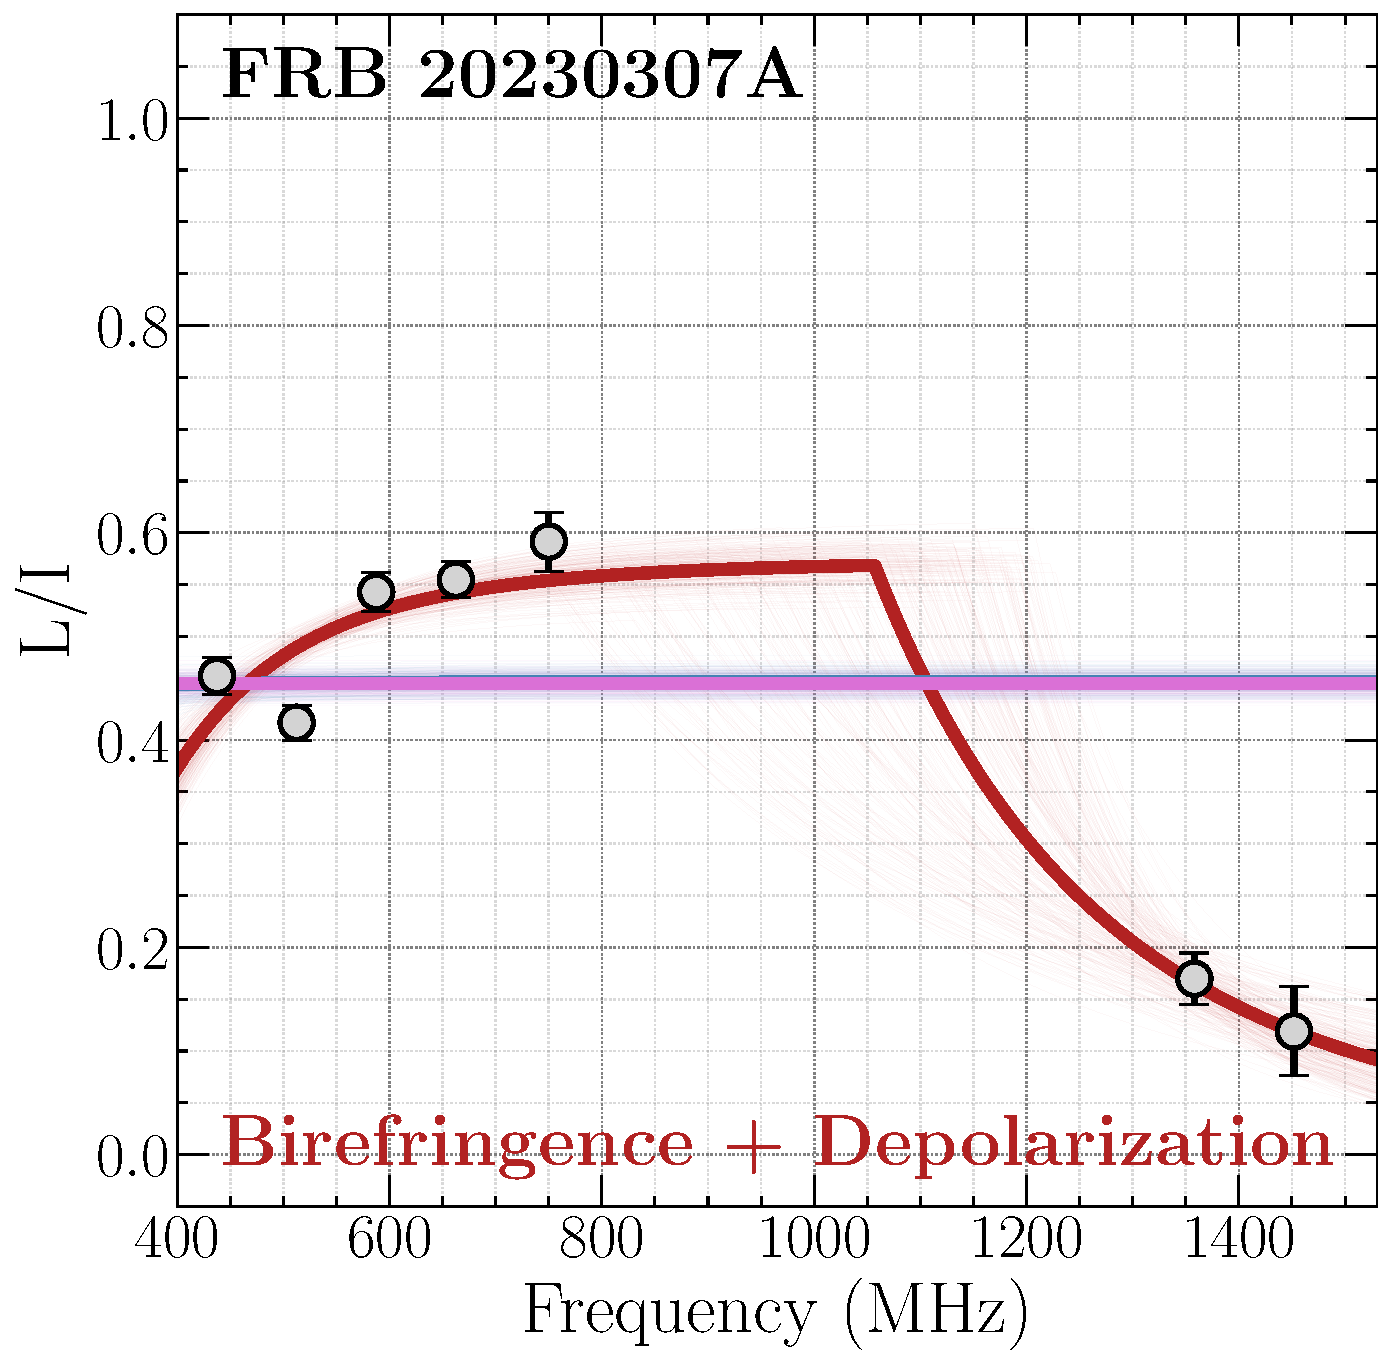
\includegraphics[width=0.28\textwidth]{frb_20230307a_lispectra.pdf}
    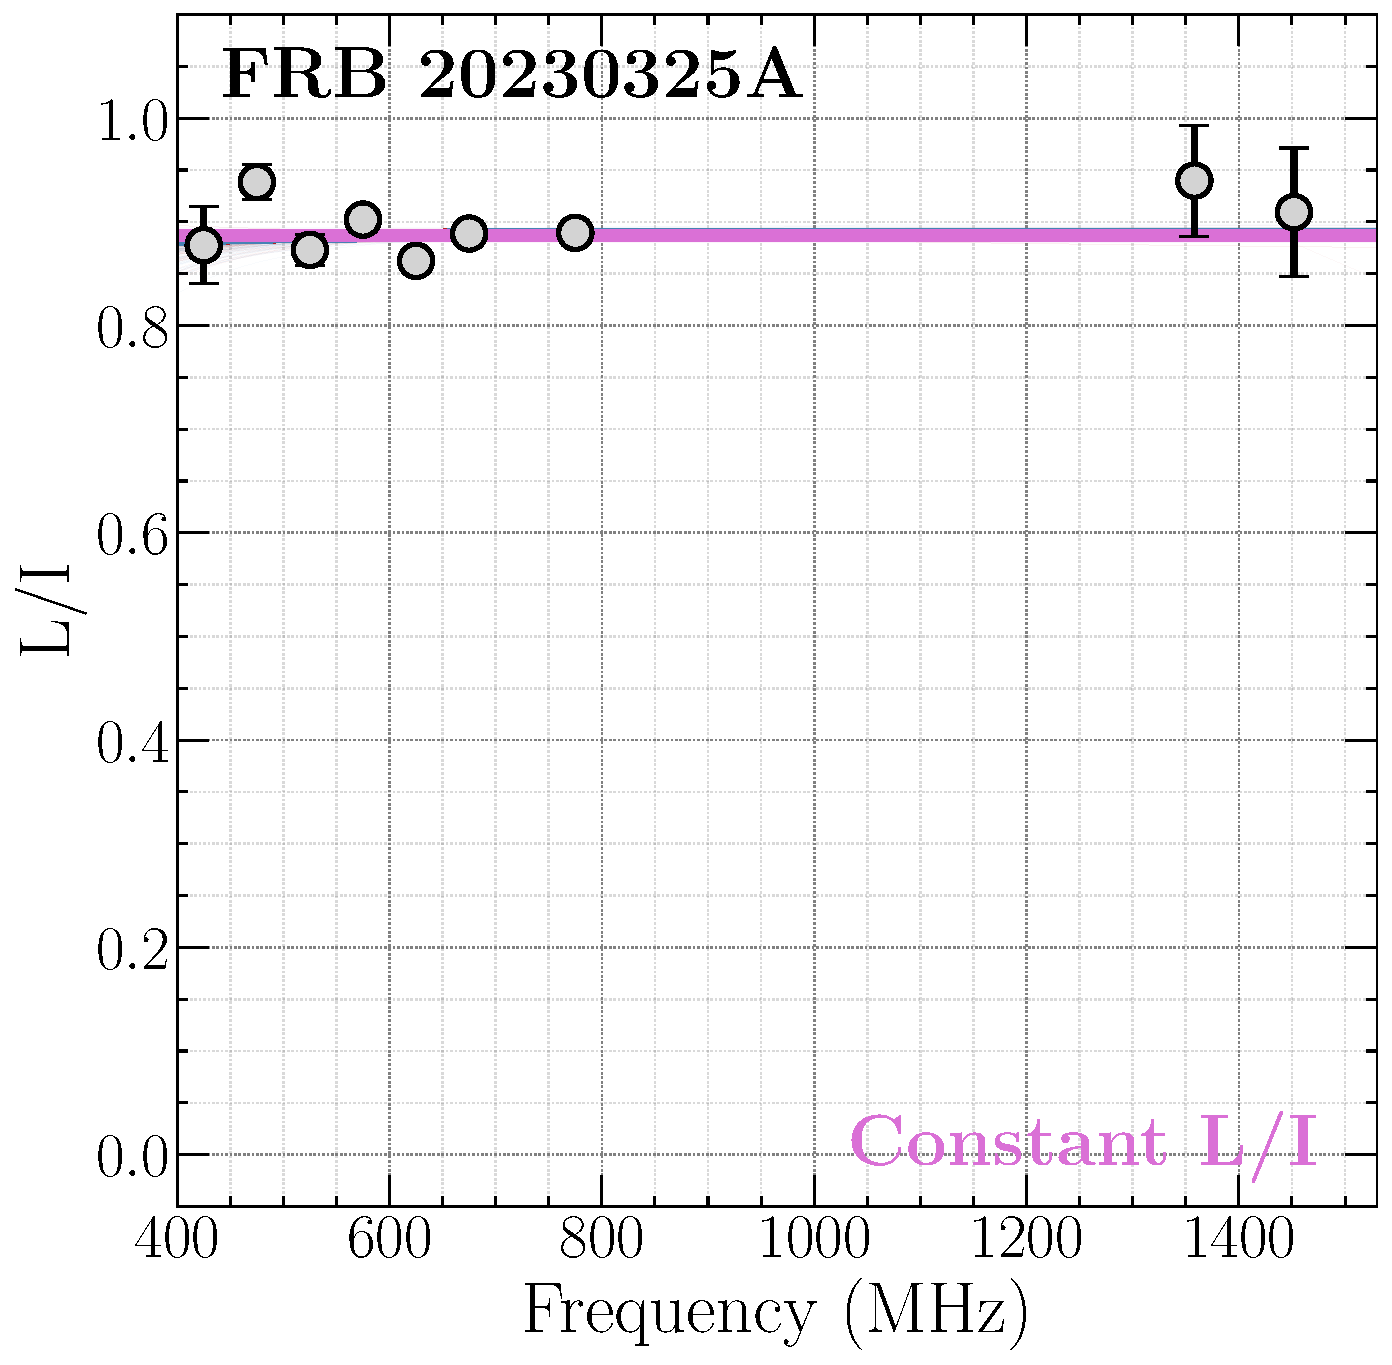
\includegraphics[width=0.28\textwidth]{frb_20230325a_lispectra.pdf}
    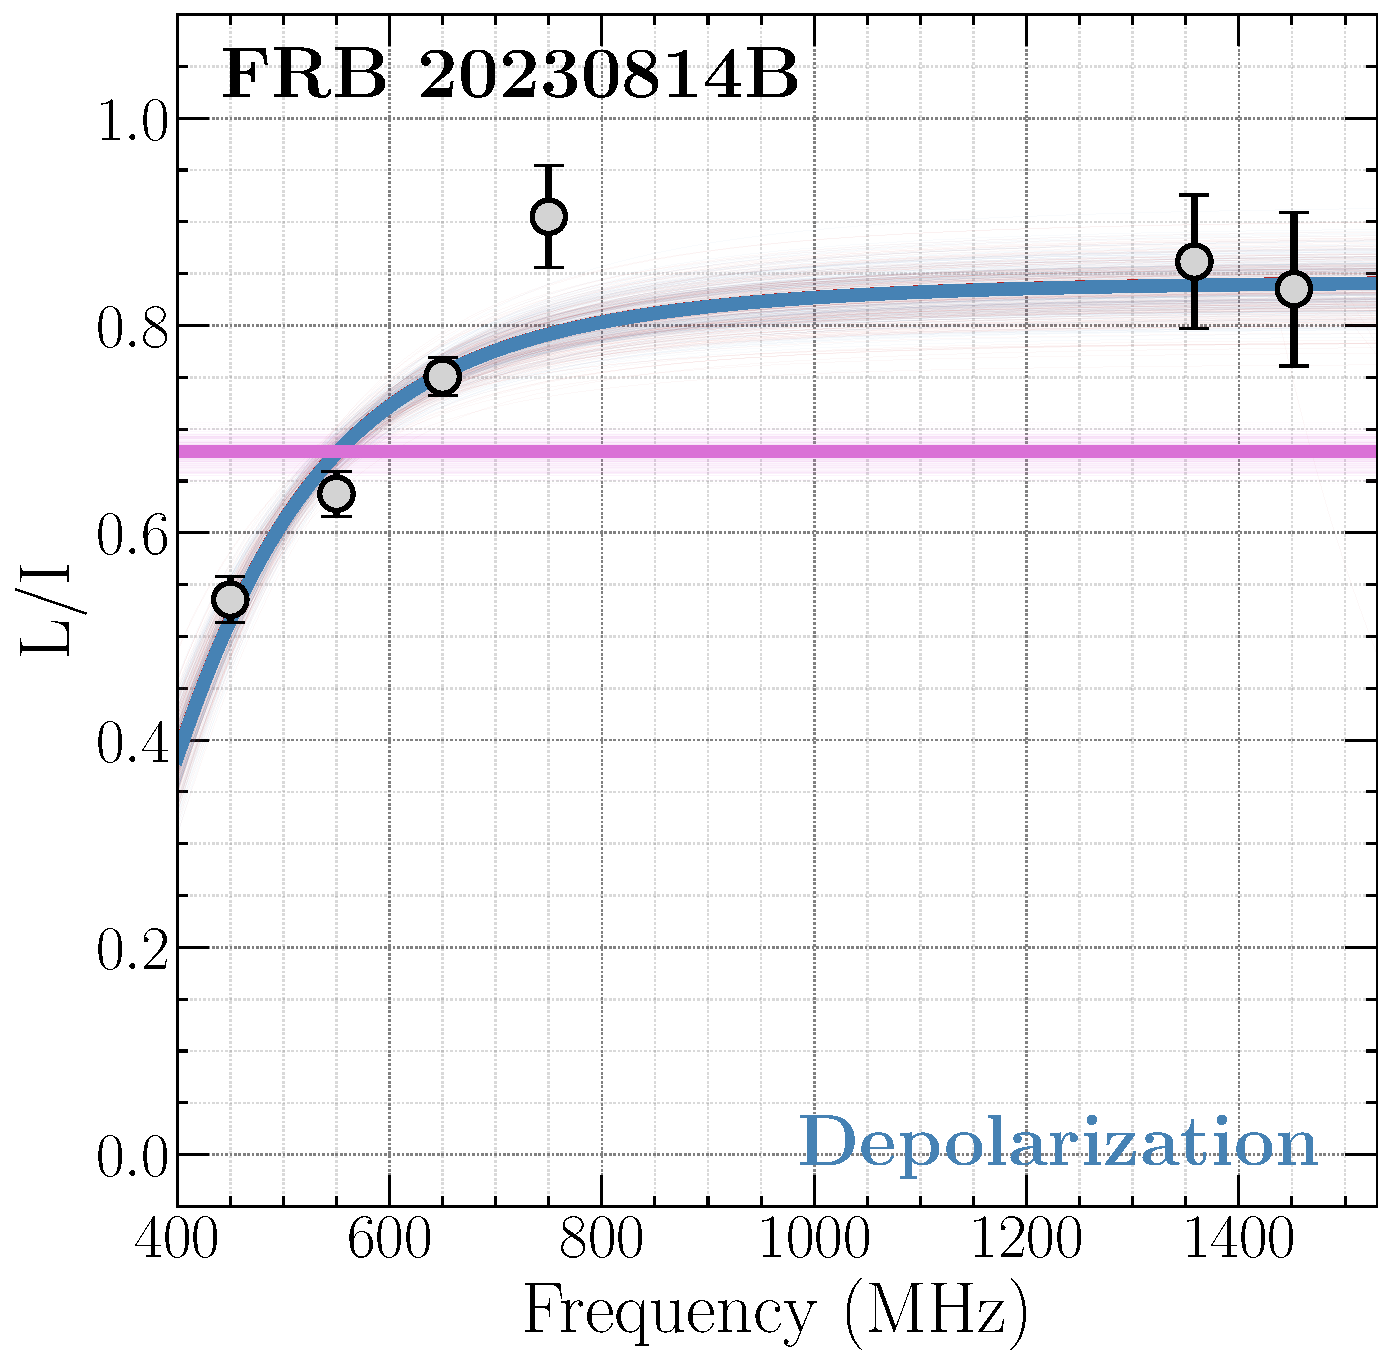
\includegraphics[width=0.28\textwidth]{frb_20230814b_lispectra.pdf}
    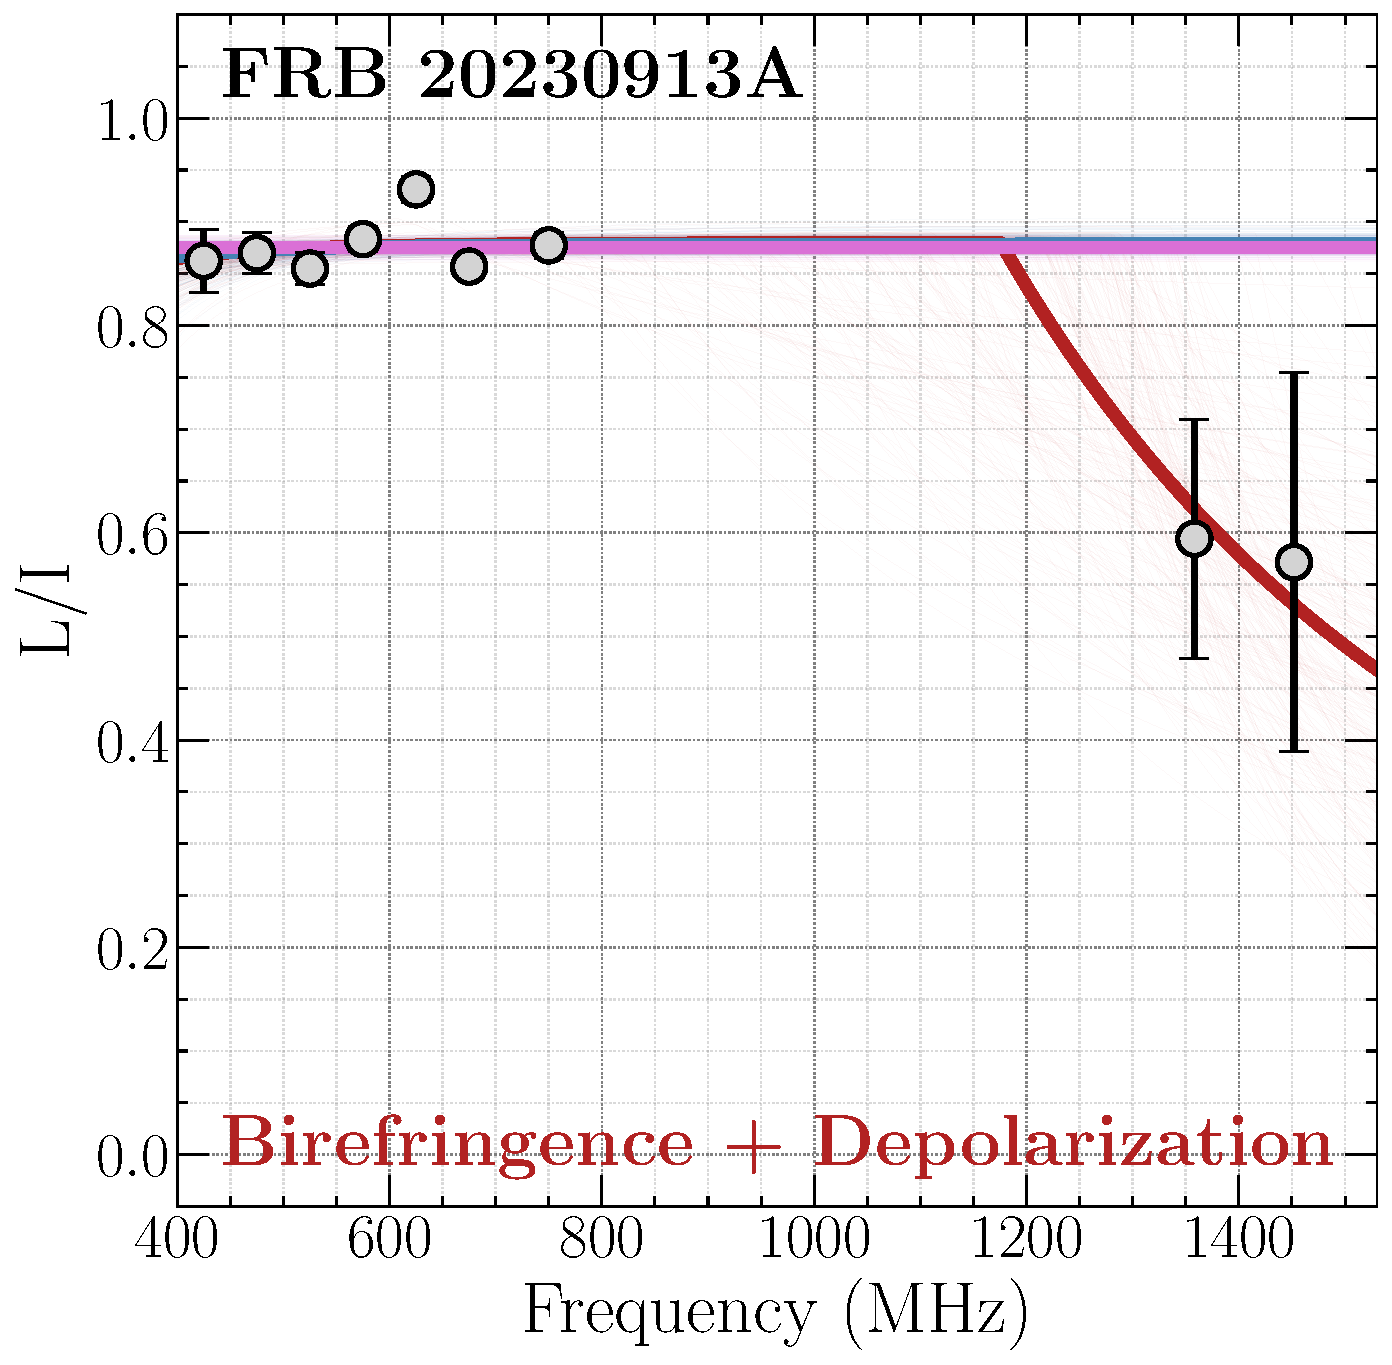
\includegraphics[width=0.28\textwidth]{frb_20230913a_lispectra.pdf}
    %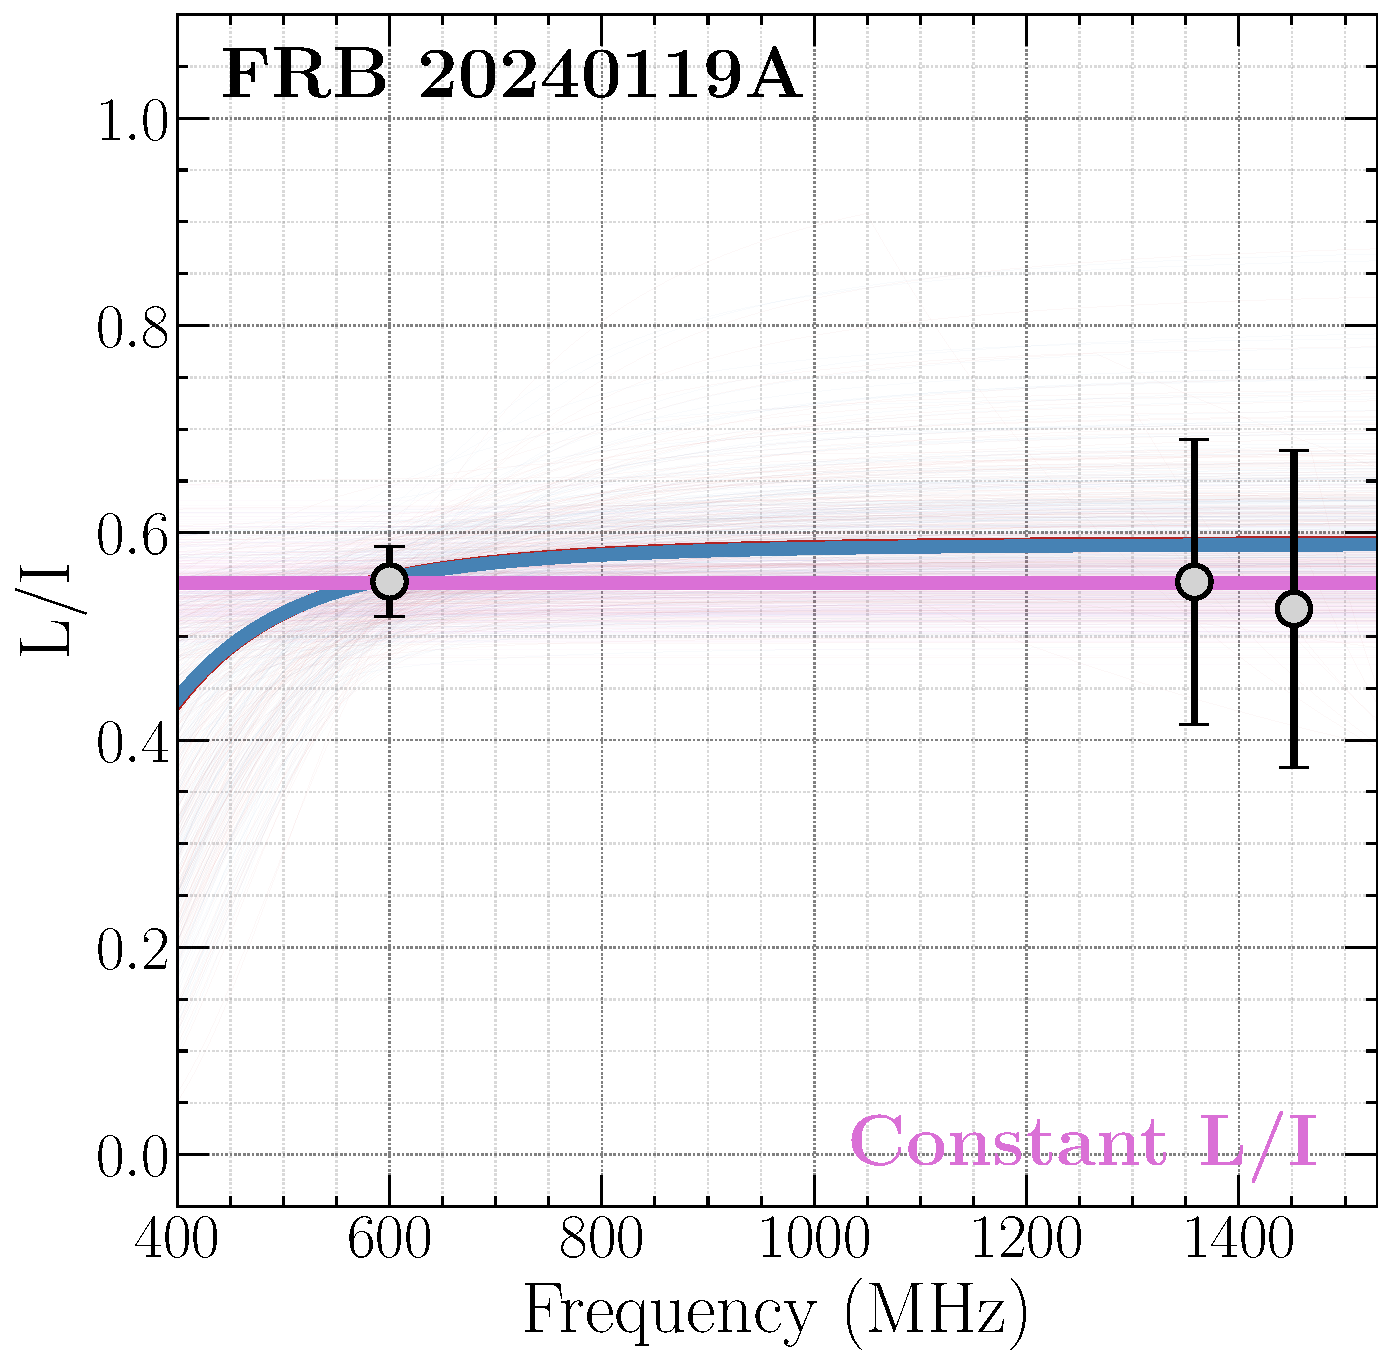
\includegraphics[width=0.28\textwidth]{frb_20240119a_lispectra.pdf}
    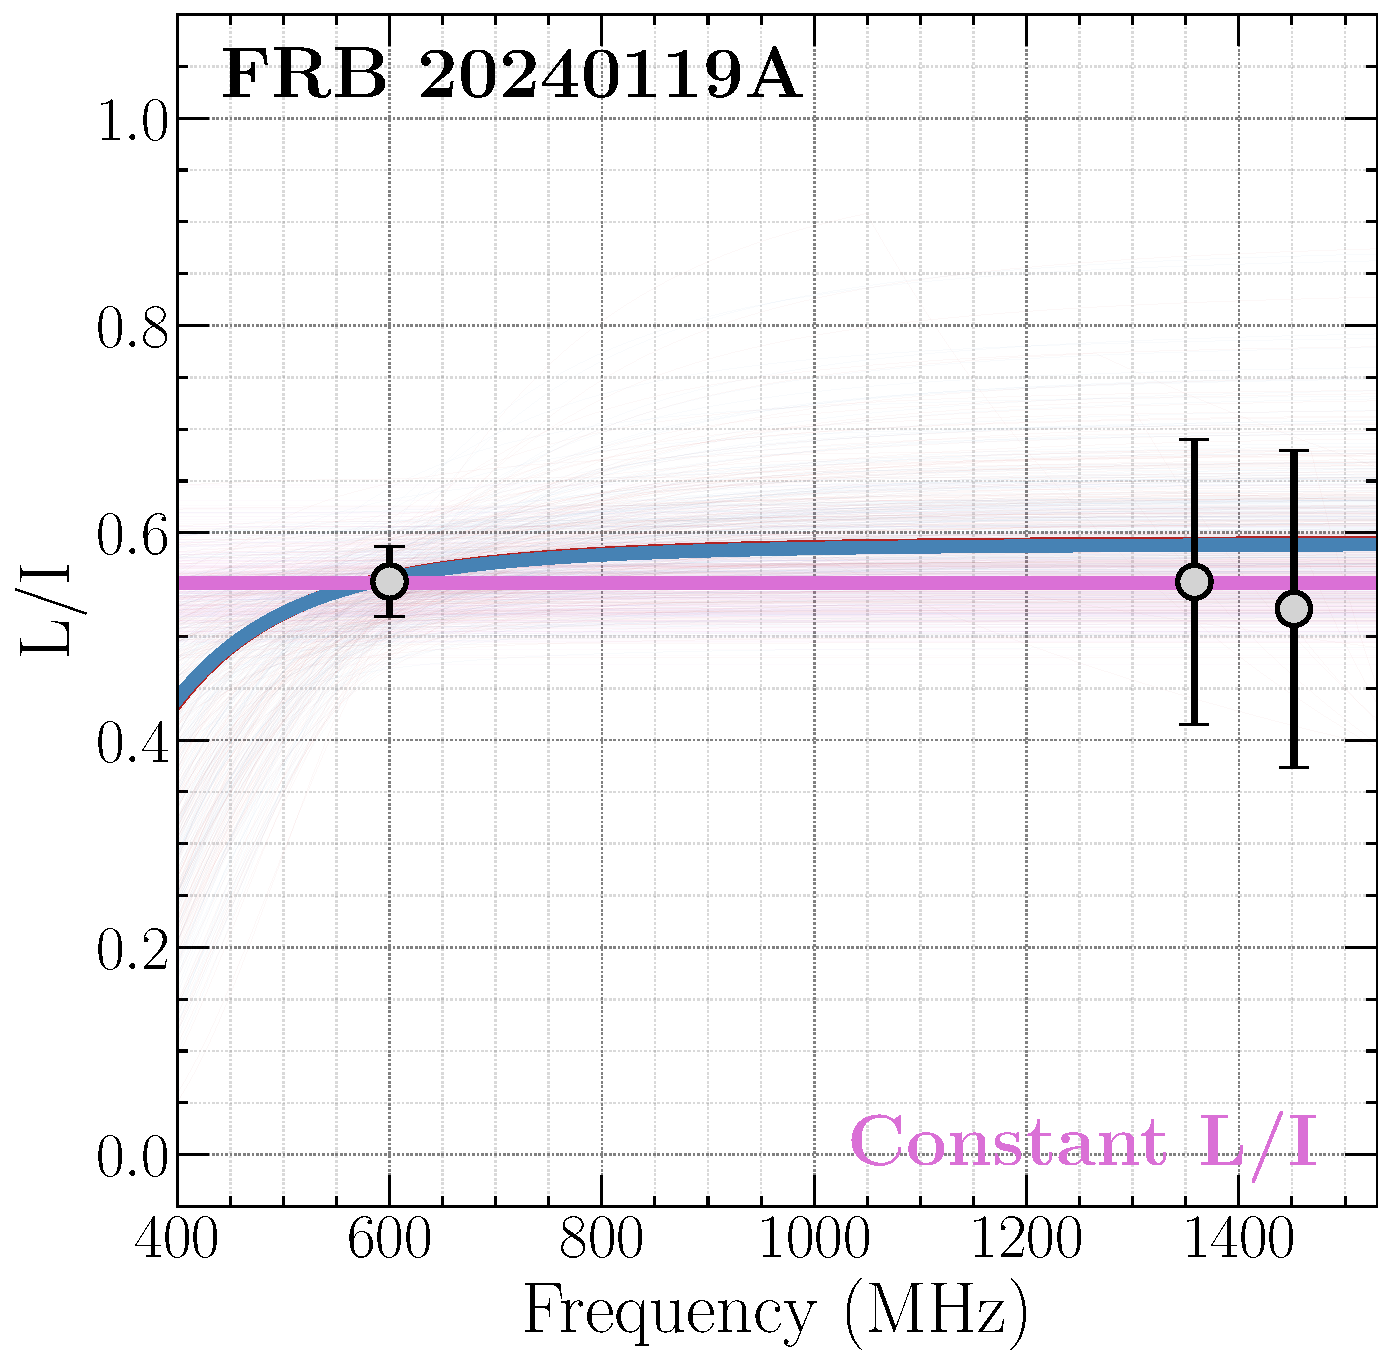
\includegraphics[width=0.28\textwidth]{frb_20240122a_lispectra.pdf}
    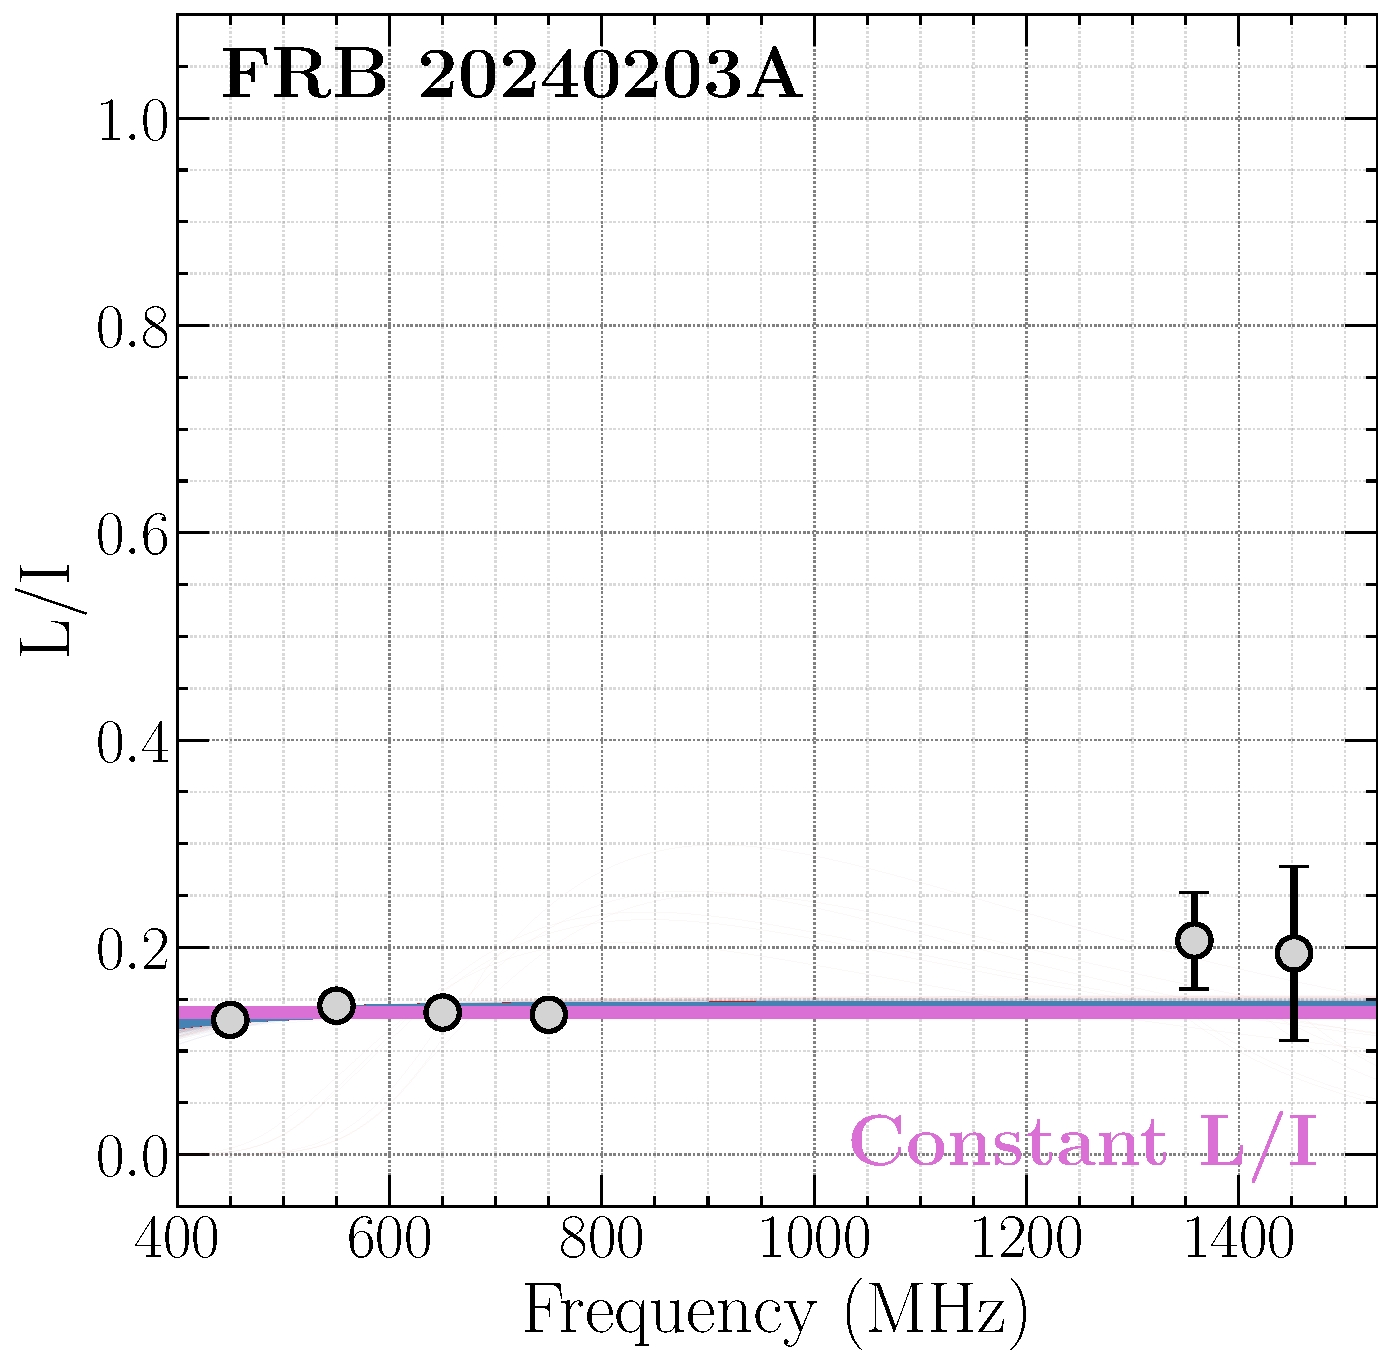
\includegraphics[width=0.28\textwidth]{frb_20240203a_lispectra.pdf}
    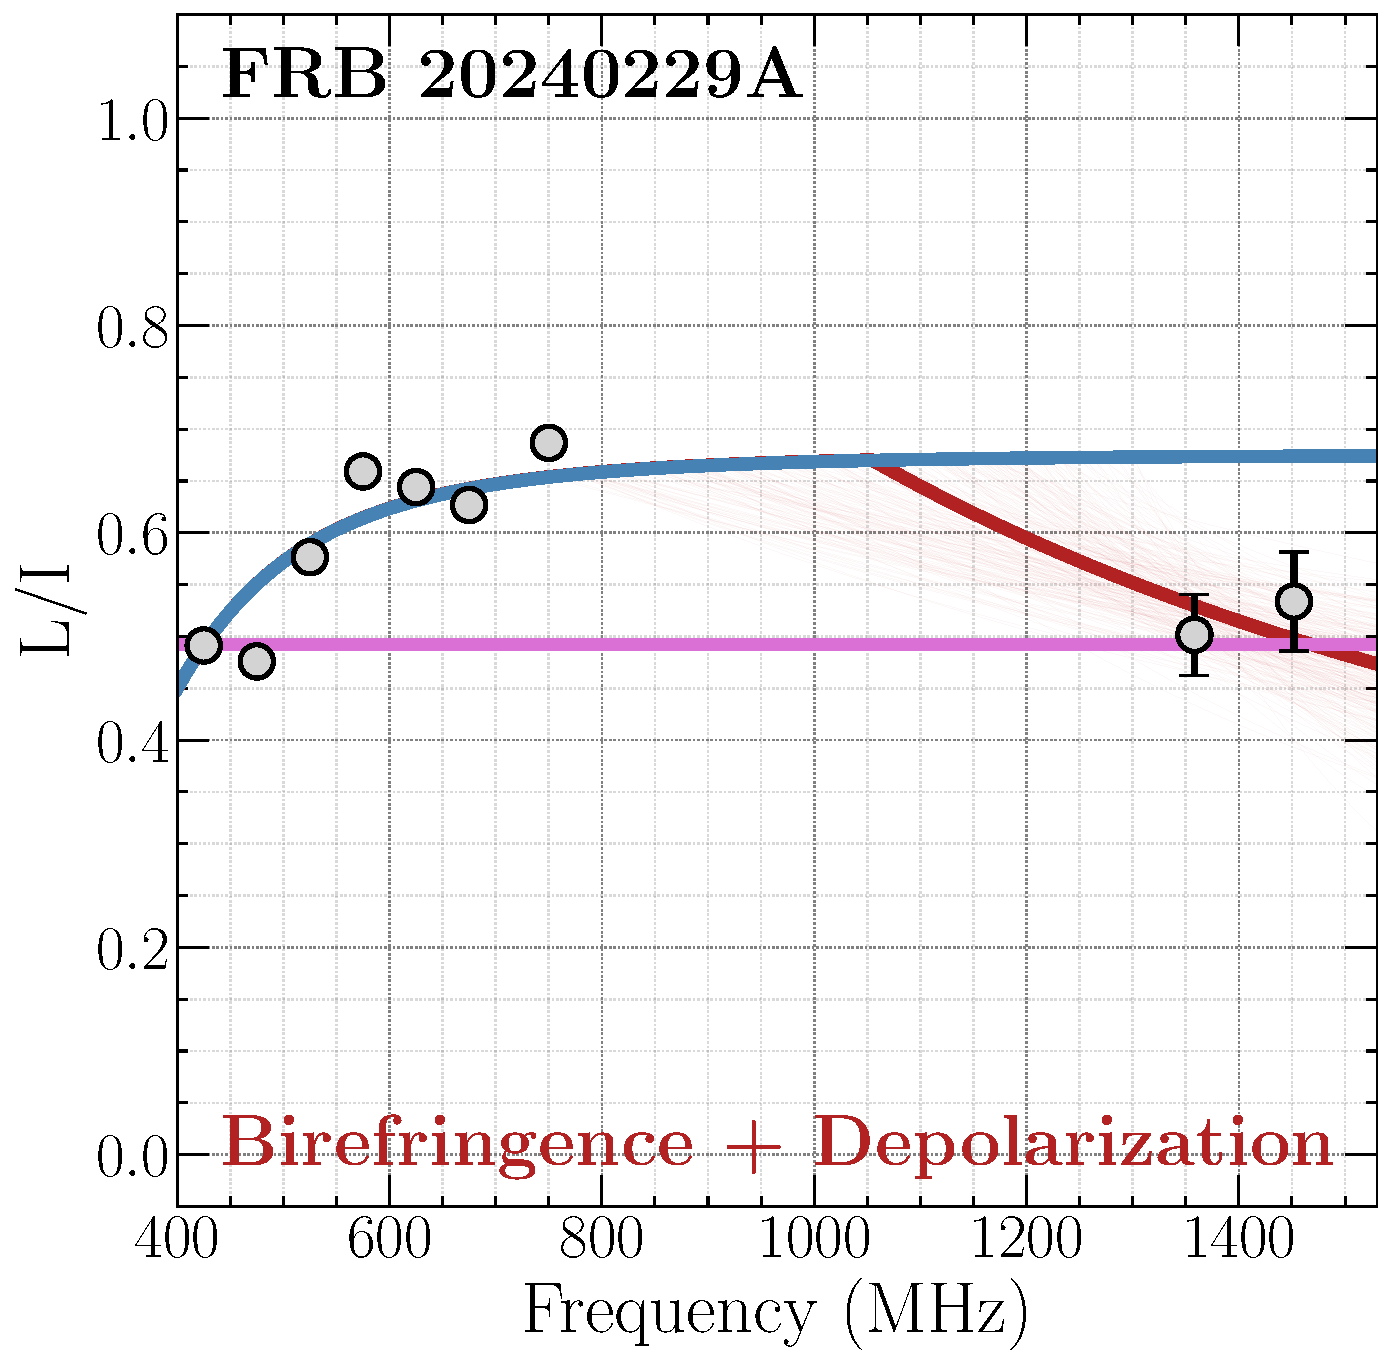
\includegraphics[width=0.28\textwidth]{frb_20240229a_lispectra.pdf}
    \caption{$L/I$ spectra across $400 - 1530$~MHz for the 12 codetected FRBs (plotted as grey circles). Models following Equations \ref{eq:model_1}, \ref{eq:model_2}, and \ref{eq:model_3} fit to each spectra are plotted as purple, blue, and red solid lines, respectively. Individual MCMC trial fits are plotted as thinner, translucent lines in the background. The best-fit model is labeled in the bottom right of each panel.} 
    \label{fig:li_spectra}
\end{figure*}

\setlength{\tabcolsep}{12.6pt}
\setlength\extrarowheight{2pt}
\setlength{\LTcapwidth}{1.0\textwidth}
\begin{table*}[t!]
\begin{center}
\caption{Summary of best-fit parameters from $L/I$ spectra modeling.} \label{tb:model_params}
\begin{tabular}{cccccc}
\hline
\hline
TNS Name & Best-fit model & $(L/I)_\mathrm{int}$ & $\sigma_\mathrm{RM}$ & $\nu_c$ & $\alpha$\\
 &  &  & (rad m$^{-2}$) & (MHz) & \\
\hline
FRB~20220207C & Depolarization & $0.862^{+0.03}_{-0.03}$ & $0.946^{+0.008}_{-0.008}$ & $-$ & $-$\\
FRB~20220310F & Constant $L/I$ & $0.56^{+0.01}_{-0.01}$ & $-$ & $-$ & $-$\\
FRB~20220506D & Depolarization & $0.92^{+0.05}_{-0.08}$ & $>3.4^{+0.2}_{-0.2}\tablenotemark{a}$ & $-$ & $-$\\
FRB~20221113A & Depolarization & $0.993^{+0.005}_{-0.010}$ & $1.30^{+0.04}_{-0.04}$ & $-$ & $-$\\
FRB~20221203A & Depolarization & $0.991^{+0.006}_{-0.010}$ & $>1.20^{+0.04}_{-0.05}\tablenotemark{a}$ & $-$ & $-$\\
FRB~20230307A & Birefringence + Depolarization & $0.57^{+0.02}_{-0.02}$ & $0.82^{+0.08}_{-0.08}$ & $1057^{+108}_{-177}$ & $-5^{+2}_{-3}$\\
FRB~20230325A & Constant $L/I$ & $0.887^{+0.002}_{-0.002}$ & $-$ & $-$ & $-$\\
FRB~20230814B & Depolarization & $0.844^{+0.02}_{-0.02}$ & $1.12^{+0.06}_{-0.07}$ & $-$ & $-$\\
FRB~20230913A & Birefringence + Depolarization & $0.880^{+0.007}_{-0.006}$ & $0.2^{+0.1}_{-0.1}$ & $1176^{+125}_{-271}$ & $-2^{+2}_{-3}$\\
FRB~20240122A & Constant $L/I$ & $0.55^{+0.03}_{-0.03}$ & $-$ & $-$ & $-$\\
FRB~20240203A & Constant $L/I$ & $0.137^{+0.002}_{-0.002}$ & $-$ & $-$ & $-$\\
FRB~20240229A & Birefringence + Depolarization & $0.676^{+0.002}_{-0.002}$ & $0.803^{+0.03}_{-0.03}$ & $1054^{+150}_{-191}$ & $-1.0^{+0.4}_{-0.9}$\\
\hline
\hline
\end{tabular}
\end{center}
\tablenotetext{$a$}{The lowest frequency bin, in which most of the depolarization occurs, is an upper limit on $L/I$, thus only a $\sigma_\mathrm{RM}$ lower limit is provided by the model fitting.}
\end{table*}

\subsection{Polarization angle} \label{sec:results_pa} 
We find that two FRBs in our sample (FRBs~20220310F and 20230814B) have variable PA profiles as a function of frequency; both of their PA profiles, integrated over multiple frequency ranges between $400-1530$~MHz, are presented in Figure \ref{fig:pa_profiles}. FRB~20220310F shows a $\sim70^\circ$ PA swing over $\sim 0.1$~ms at $1280-1530$~MHz, which is reduced to a flat PA profile spanning $\sim 1$~ms with a maximum PA variation of only $\sim 30^\circ$. At $1280-1530$~MHz, FRB~20230814A shows a $\sim 50^\circ$ PA swing over $\sim 0.1$~ms. Dividing the CHIME/FRB band in two, we find that the maximum PA variation is reduced to $\sim 20^\circ$ at $600-800$~MHz, and further to $\sim 10^\circ$ at $400-600$~MHz. Most of the remaining $10/12$ FRBs in our sample show flat PA profiles at both CHIME/FRB and DSA-110 frequencies, and a few have such a low $S/N$ in one of the two datasets that we cannot construct a robust PA profile over multiple frequency bands.

\begin{figure}
    \centering
    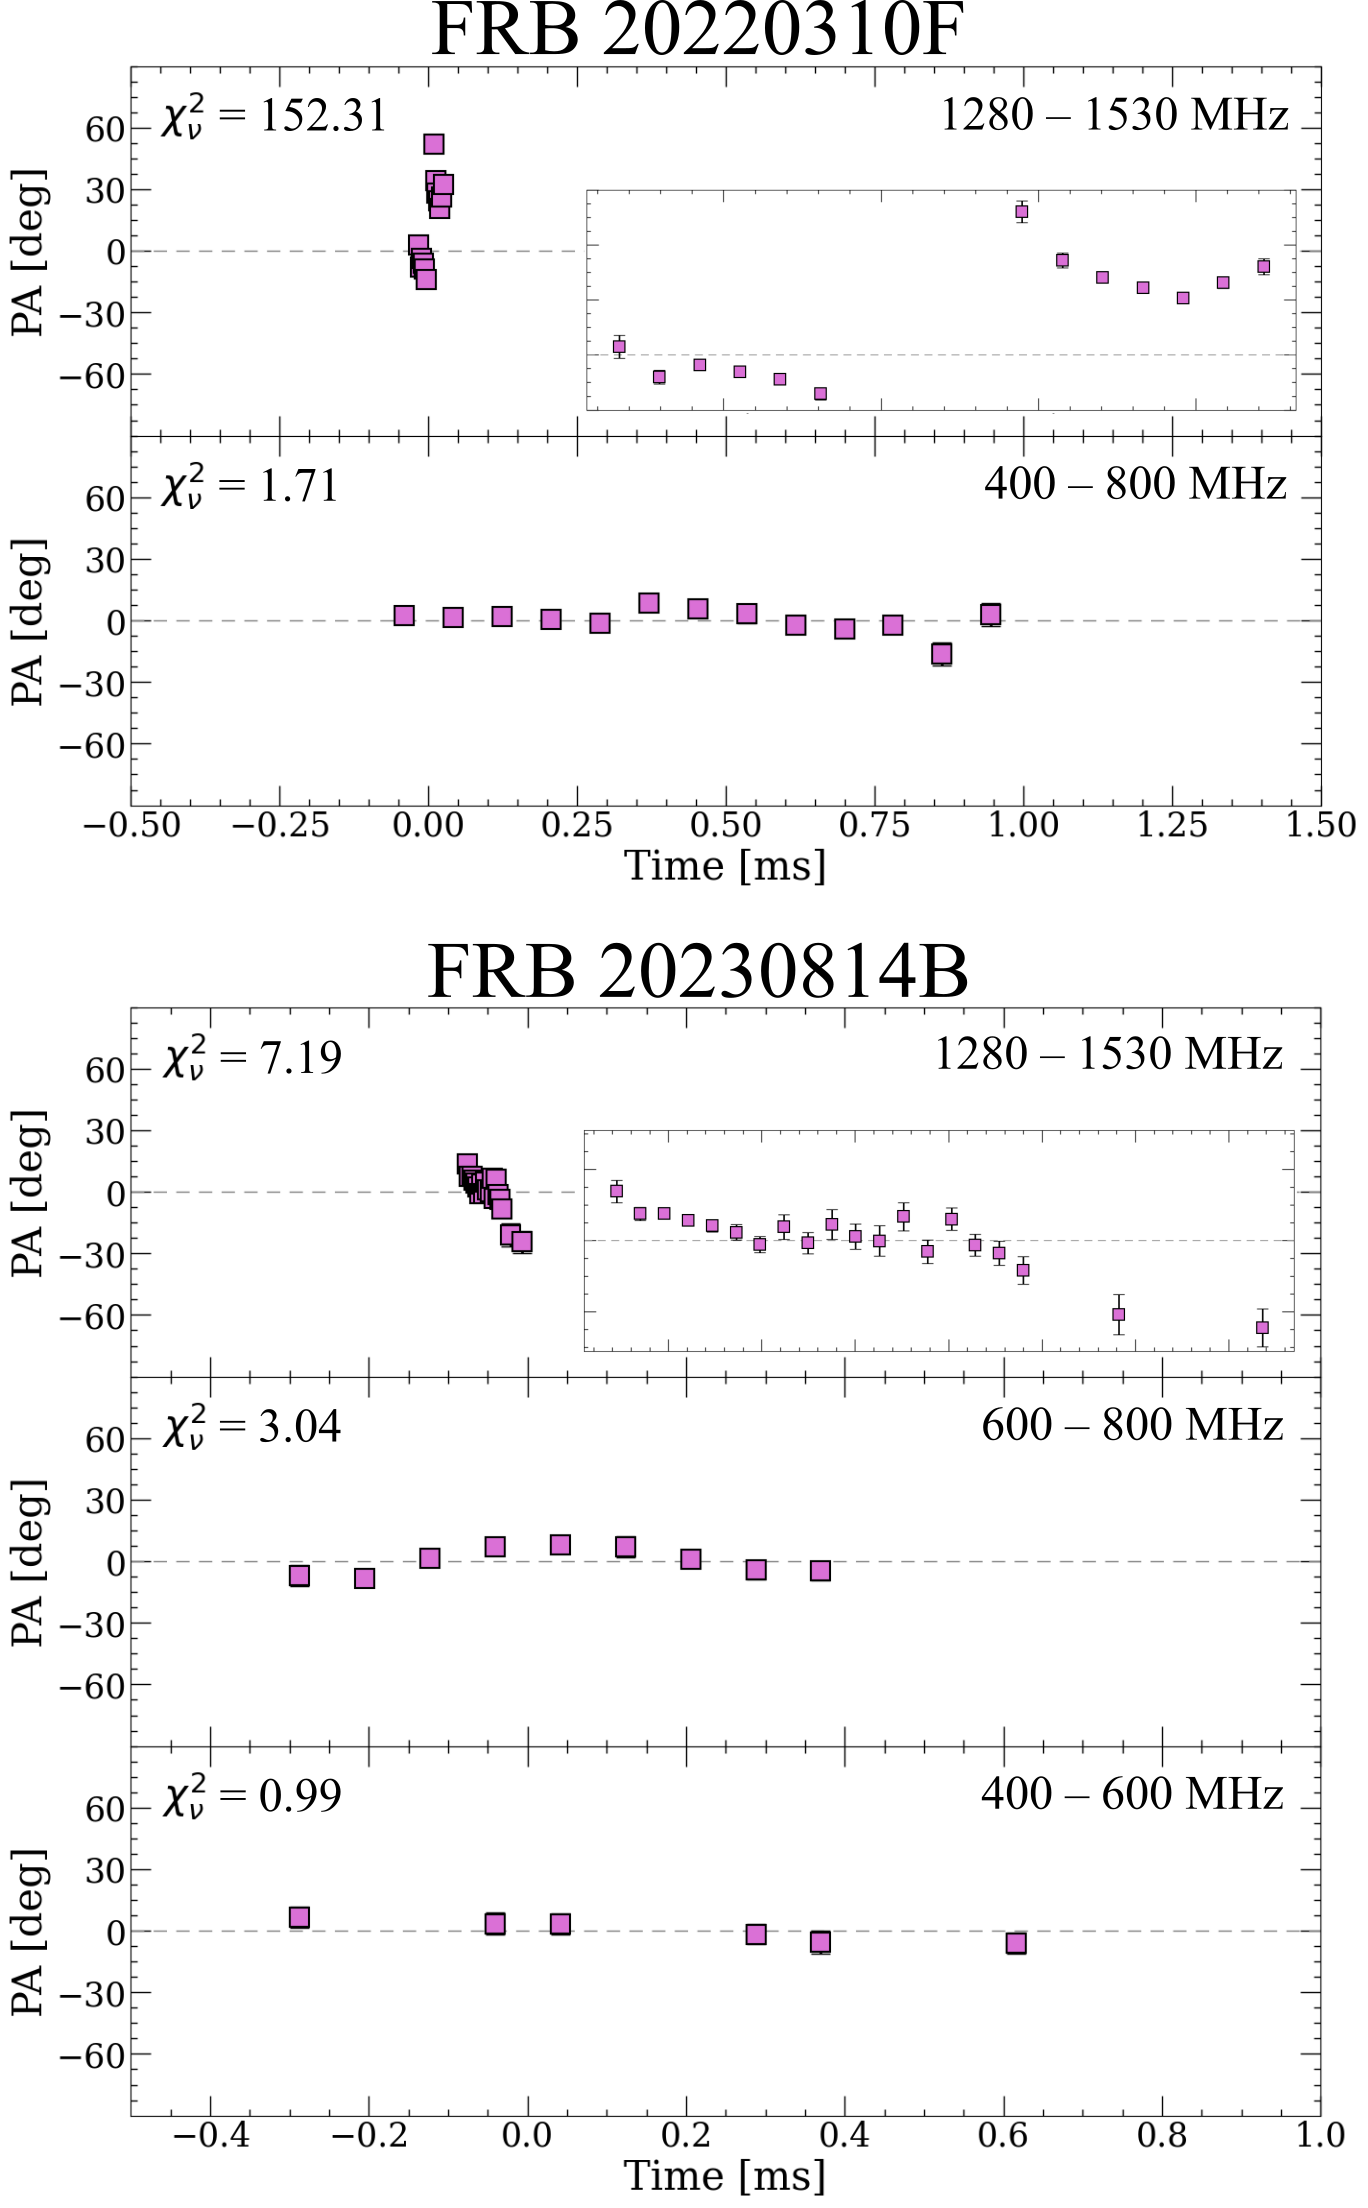
\includegraphics[width=0.47\textwidth]{pa_flattening_profiles.png}
    \caption{(Top) Temporal PA profile of FRB~20220310F integrated over $1280-1530$~MHz and $400-800$~MHz. The reduced chi squared, $\chi_\nu^2$, from comparing the PA profiles to a constant PA of $0^\circ$ is presented in the top left of each panel. An inset showing the zoomed in (spanning $\sim 0.1$~ms) PA profile at the higher-frequency band is overplotted in the first panel. (Bottom) The same plot but for FRB~20230814B. The CHIME/FRB detection of this burst has sufficient linearly polarized intensity to divide the data into two subbands, thus PA profiles integrated over $400-600$~MHz and $600-800$~MHz are presented.} 
    \label{fig:pa_profiles}
\end{figure}

\subsection{Correlation between depolarization, Faraday rotation, and scattering} \label{sec:results_depol}
Correlations between $\sigma_\mathrm{RM}$, $|\mathrm{RM}|$, and scattering time scale ($\tau$) have been suggested as signposts for FRBs originating in dense, magnetized, and inhomogeneous environments. However, the significance of these correlations have only been marginal thus far, chiefly owing to the small sample size of depolarizing FRBs \citep{2022Sci...375.1266F, 2025MNRAS.tmp.1894U, 2026ApJ..1000L..53P}. Here, we revisit the $\sigma_\mathrm{RM}-|\mathrm{RM}|$ and $\sigma_\mathrm{RM}-\tau$ relationships with all depolarizing FRBs in the literature in addition to the five FRBs in this work that show evidence for depolarization, have measured scattering timescales, and are associated with host galaxies with spectroscopic redshifts (FRBs~20220207C, 20221113A, 20230307A, 20230814B, and 20240229A; for measurements of their scattering timescales and host galaxy associations, see paper I).

We follow the steps described by \cite{2026ApJ..1000L..53P} to evaluate these correlations, specifically accounting for a conversion to the FRB rest-frame and for RM variability in some repeating FRBs. First, we convert to the rest-frame RM scatter, $\sigma_\mathrm{RM,host}$, given the cosmological redshift, $z$, of the FRB host galaxies \citep{2024MNRAS.528.2511T},
\begin{equation}
\sigma_\mathrm{RM,host} = \sigma_\mathrm{RM} (1+z)^2\,. \label{eq:sigma_rm_host}
\end{equation}
Following Equation \ref{eq:rm_comps}, we assume $\mathrm{RM}_\mathrm{ion} = \mathrm{RM}_\mathrm{IGM} = 0~\mathrm{rad}~\mathrm{m}^{-2}$, subtract the Galactic RM as measured by \cite{2022A&A...657A..43H}, convert to the rest frame by applying a $(1+z)^2$ correction factor, and the the absolute value to get $|\mathrm{RM}_\mathrm{host}|$. If the source is a repeating FRB, we take the median of $|\mathrm{RM}_\mathrm{host}|$ across all polarized bursts.

In the left panel of Figure \ref{fig:sigmarm_correlation}, we plot the $|\mathrm{RM}_\mathrm{host}|$ versus $\sigma_\mathrm{RM,host}$ of depolarizing FRBs in this work compared to other known depolarizing FRBs \citep{2022Sci...375.1266F, 2025MNRAS.tmp.1894U, 2026ApJ..1000L..53P}. For the repeating FRBs, we plot the 68\% confidence interval around the median $|\mathrm{RM}_\mathrm{host}|$ as shaded regions. We undertake a Pearson R test on the $\mathrm{log}_{10}(\sigma_\mathrm{RM,host})-\mathrm{log}_{10}(|\mathrm{RM}_\mathrm{host}|)$ relationship, finding a test statistic equal to $0.764$ (positive correlation) with a p-value of $0.001$ ($\sim 3.2 \sigma$). Thus, we consider this correlation to be statistically significant.

Next, we restrict our depolarizing FRB sample to only those with measured scattering timescales exceeding the contribution predicted by the NE2025 model \citep[scaled to the same reference frequency assuming a frequency dependence of $\nu^{-4}$;][]{2026arXiv260211838O} by more than an order of magnitude \citep{2019MNRAS.486.3636P, 2022ApJ...927...59L, 2023MNRAS.519..821O, 2025ApJ...992..206C, 2025PASA...42..133S}. Assuming negligible scattering contributing from any intervening galaxy halos, enforcing this threshold allows us to have a high level of confidence that the observed scattering timescales are dominated by contributions from the FRB host galaxy or immediate environment. After this cut, we retain all of the depolarizing FRBs in this work and $7/9$ of the depolarizing FRBs in the literature. Converting the scattering timescale to the FRB rest frame to account for cosmological time dilation, assuming $\tau \propto \nu^{-4}$, we apply the equation
\begin{equation}
\tau_\mathrm{host} = \tau/(1+z)^3\,, \label{eq:tau_host}
\end{equation}
\citep{Macquart_2013_ApJ}. Note that if the scattering index diverges from the assumed $\nu^{-4}$, it can change the significance of any observed correlation. In the middle panel of Figure \ref{fig:sigmarm_correlation}, we plot $\tau_\mathrm{host}$ versus $\sigma_\mathrm{RM,host}$ of depolarizing FRBs. Again, the 68\% confidence intervals around the median $\tau_\mathrm{host}$ for repeaters are plotted as shaded regions. Performing a Pearson R test on $\mathrm{log}_{10}(\sigma_\mathrm{RM,host})-\mathrm{log}_{10}(\tau_\mathrm{host})$, we find a test statistic of $0.775$ with a p-value equal to $0.003$ ($\sim 3.0 \sigma$), making this correlation statistically significant as well.

Finally, we plot $\tau_\mathrm{host}$ versus $|\mathrm{RM}_\mathrm{host}|$ (with shaded regions representing the 68\% confidence intervals for both $\tau_\mathrm{host}$ and $|\mathrm{RM}_\mathrm{host}|$ in repeaters) for all depolarizing FRBs with scattering measurements available in the right panel of Figure \ref{fig:sigmarm_correlation}. A Pearson R test conducted on $\mathrm{log}_{10}(|\mathrm{RM}_\mathrm{host}|)-\mathrm{log}_{10}(\tau_\mathrm{host})$ finds a statistically significant correlation with a test statistic of $0.869$ and p-value equal to $0.0002$ ($\sim 3.7 \sigma$).

We caution that the correlations presented above are sensitive to the inclusion of FRB~20190520B, which has $\sigma_\mathrm{RM,host}$ and $\tau_\mathrm{host}$ that are an order of magnitude or more larger than the rest of the sample. Removing FRB~20190520B and repeating the tests returns Pearson R test statistics of $0.744$ with p-value $0.004$ (for the $\mathrm{log}_{10}(\sigma_\mathrm{RM,host})-\mathrm{log}_{10}(|\mathrm{RM}_\mathrm{host}|)$ correlation), $0.528$ with p-value $0.095$ (for the $\mathrm{log}_{10}(\sigma_\mathrm{RM,host})-\mathrm{log}_{10}(\tau_\mathrm{host})$ correlation), and $0.819$ with p-value $0.002$ (for the $\mathrm{log}_{10}(|\mathrm{RM}_\mathrm{host}|)-\mathrm{log}_{10}(\tau_\mathrm{host})$ correlation). 

In Figure \ref{fig:scat_hist}, we plot the cumulative distribution function of $\tau$ (in the observer frame since not all FRBs in our sample are associated with host galaxies) for FRBs with (blue) and without (red) depolarization of their linearly polarized spectra. For comparison, we also show the distribution of $\tau$ measured in the first CHIME/FRB baseband catalog \citep{2025ApJ...979..160S}. Here, we have employed statistical methods that take censored data into account \citep[see, e.g.,][]{2012msma.book.....F}, via the {\tt NADA V1.6-1.2} package\footnote{\url{https://rdrr.io/cran/NADA/}} in {\tt R} \citep{helsel2005nondetects, NADApackage, Rsoftware}, to incorporate the $\tau$ upper limits into the empirical cumulative distribution function. While it is difficult to draw definitive conclusions due to our limited sample size, we note that FRBs undergoing depolarization peak at larger scattering timescale than those with no measurable depolarization above $400$~MHz. The mean scattering timescale, referenced to $600$~MHz, for the seven depolarizing FRBs is $\tau = 2.7\pm1.9$~ms, while the mean for FRBs without depolarization is $\tau = 1.4\pm0.3$~ms. Further, the codetected FRB sample as a whole has a larger average scattering timescale than seen in the larger CHIME/FRB population. 

\begin{figure*}
    \centering
    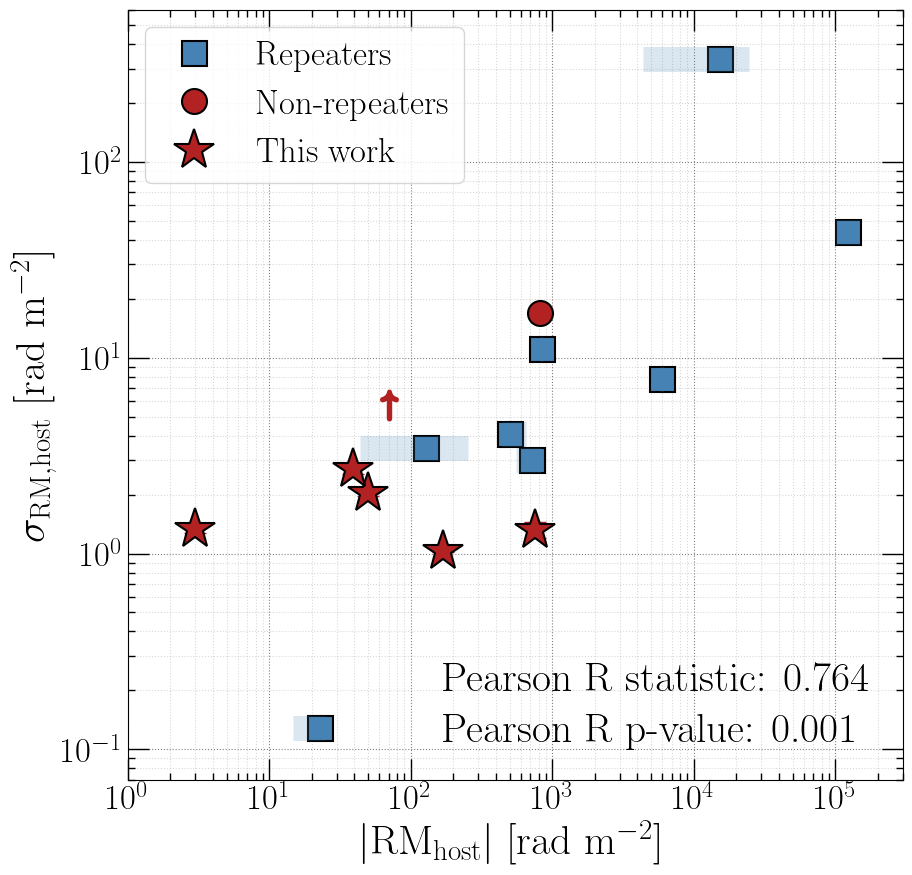
\includegraphics[width=0.325\textwidth]{sigmarm_rm.png}
    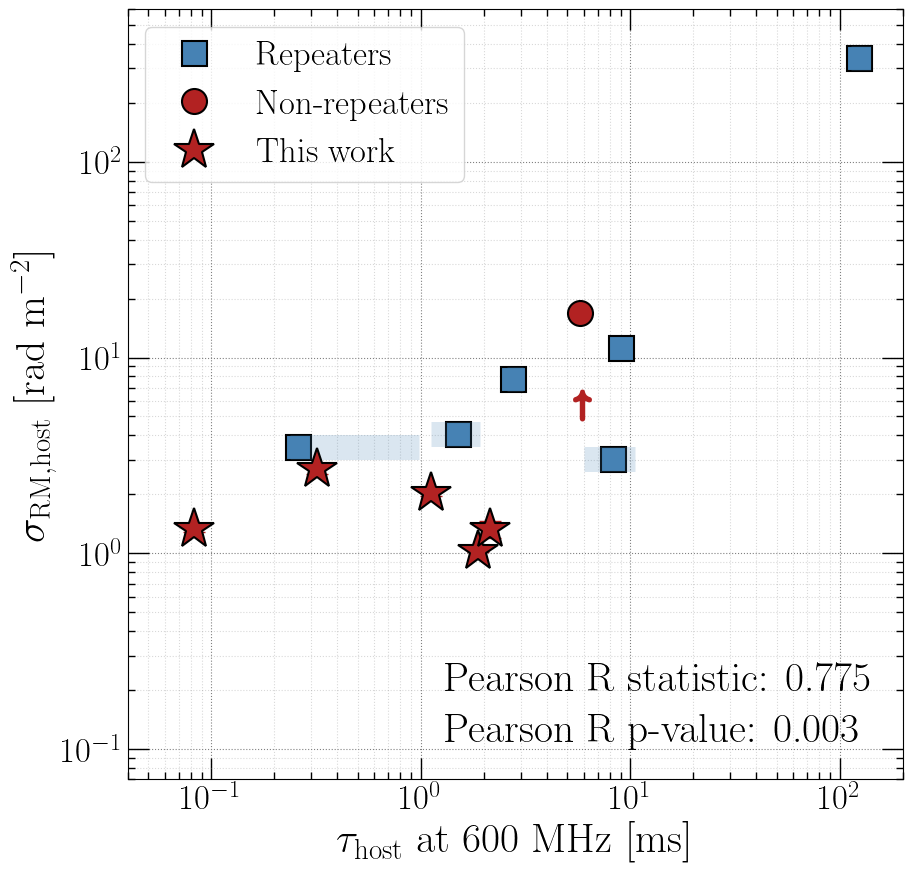
\includegraphics[width=0.325\textwidth]{sigmarm_scat.png}
    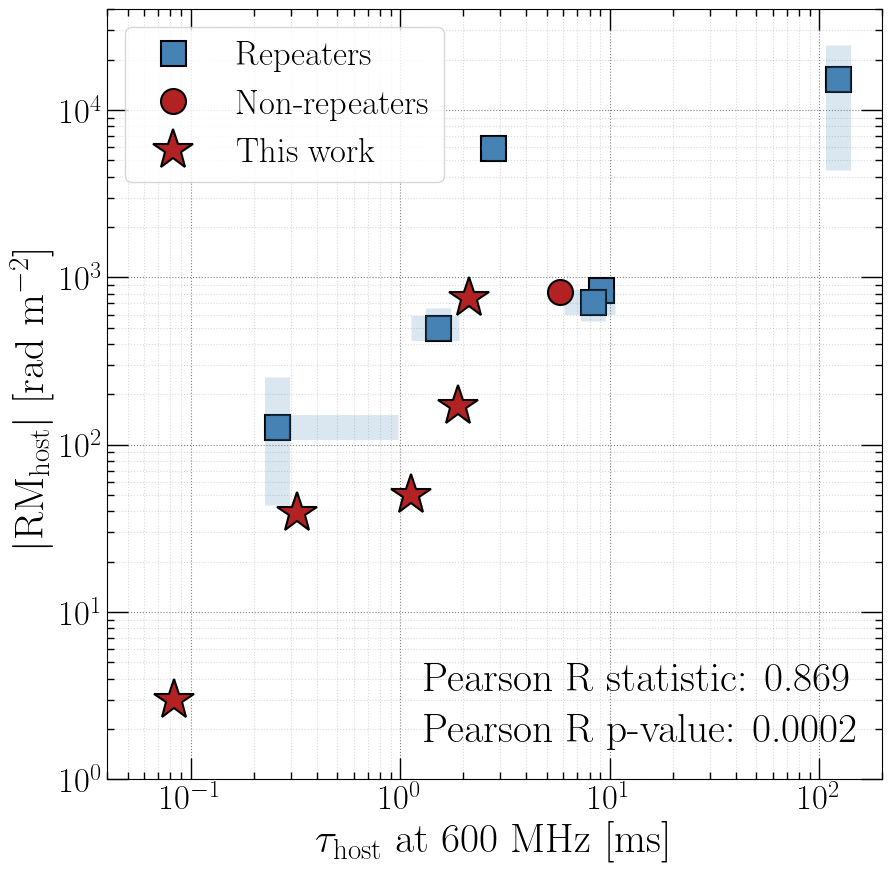
\includegraphics[width=0.318\textwidth]{scat_rm.png}
    \caption{(Left) Rest-frame scatter in the observed RM, $\sigma_\mathrm{RM,host}$, plotted as a function of $|\mathrm{RM}_\mathrm{host}|$ for the five codetected (non-repeating) FRBs that show depolarization signatures and have a host galaxy with a measured spectroscopic redshift (red stars). The $\sigma_\mathrm{RM,host}$ lower limit for FRBs~20220506D is plotted as a red arrow; we do not include FRB~20221203A as it does not have an a reliable spectroscopic redshift). Depolarizing FRBs previously identified in the literature are overplotted as blue squares \citep[repeaters;][]{2022Sci...375.1266F, 2026ApJ..1000L..53P} and red circles \citep[non-repeaters;][]{2025MNRAS.tmp.1894U}. (Middle) Similar to the left but showing rest-frame scattering timescale referenced to 600~MHz, where available, versus $\sigma_\mathrm{RM,host}$ for the same sample of FRBs. (Right) Rest-frame scattering timescale referenced to 600~MHz versus $|\mathrm{RM}_\mathrm{host}|$ for the same sample as the middle panel. Blue shaded regions in all panels represent the 68\% confidence interval around the median $|\mathrm{RM}_\mathrm{host}|$ and $\tau$ for repeaters, respectively. Uncertainties on $\sigma_\mathrm{RM,host}$ are smaller than the markers. The test statistics and p-values from Pearson R tests in all cases are presented in the bottom right of each panel.} 
    \label{fig:sigmarm_correlation}
\end{figure*}

\begin{figure}
    \centering
    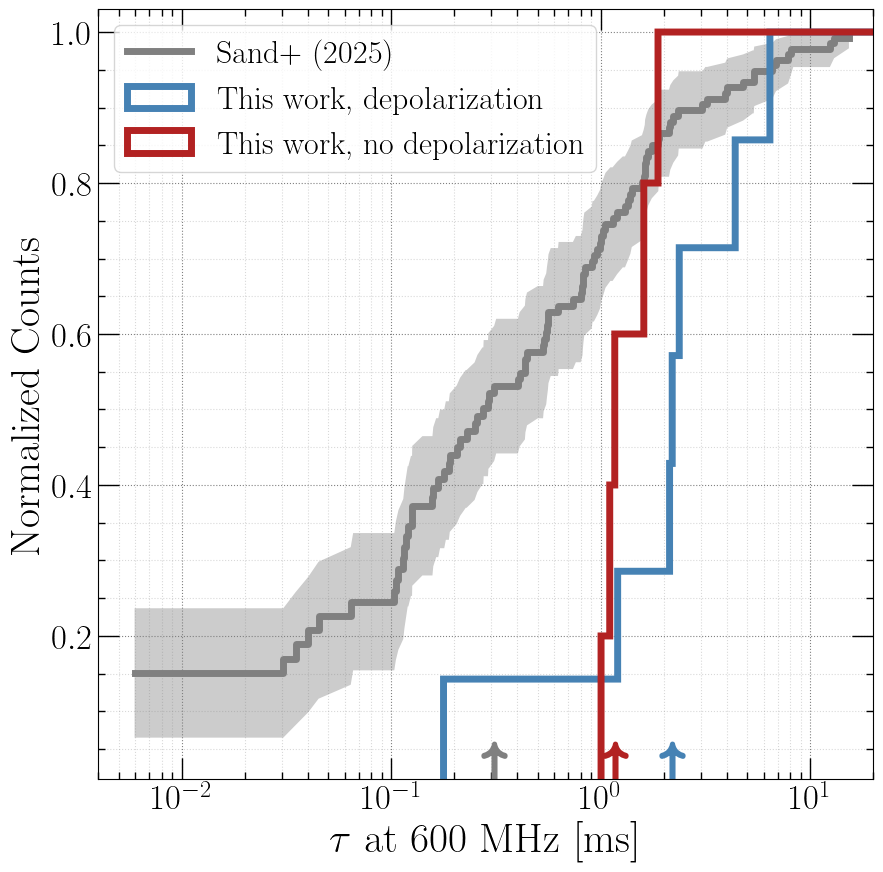
\includegraphics[width=0.47\textwidth]{scat_depol_vs_nodepol.png}
    \caption{Cumulative distribution function of the scattering timescale (observer frame and referenced to $600$~MHz) of the seven depolarizing (blue) and five non-depolarizing (red) codetected FRBs. The median of each distribution is marked by an upward-facing arrow in their respective colors. Overplotted in gray is the empirical cumulative distribution function of scattering timescales for the $137$ FRBs from the first CHIME/FRB baseband catalog \citep{2025ApJ...979..160S}. For this data, lower limits have been incorporated as censored data and the shaded region represents the 95\% confidence interval.} 
    \label{fig:scat_hist}
\end{figure}

\section{Discussion} \label{sec:discussion}
Our unique observing frequency coverage obtained from codetections of FRBs between CHIME/FRB and DSA-110 provides both broadband and low frequency observations that enable the characterization of spectropolarimetric propagation effects that are, thus far, underexplored in FRBs. Namely, we find that only a third ($4/12$ sources) of our FRB sample exhibits constant $L/I$ as a function of frequency, as would be expected for FRB emission that is not strongly distorted by propagation effects in the immediate source environment. Instead FRBs commonly show evidence for depolarization towards $400$~MHz ($7/12$ sources), and $3/12$ sources show an increase in $L/I$ from the DSA-110 band to the CHIME/FRB band. A suppression of PA variability is also observed in two sources that exhibit clear PA swings at $1400$~MHz and appear to have constant PA profiles at $400-800$~MHz, where scatter broadening is more prominent. While these propagation effects are seen in a large portion of our codetected sample, these FRB sources do not otherwise appear to be originating from noteworthy local environments \citep[i.e., their $\mathrm{DM}_\mathrm{host}$, $\mathrm{RM}_\mathrm{host}$, and $\left<B_{\parallel,\mathrm{host}}\right>$ are typical compared to the polarized FRB populations observed by CHIME/FRB and DSA-110;][]{2024ApJ...968...50P, 2024ApJ...964..131S}, suggesting that these spectral features may be common among the FRB population. In this section, we interpret the physical origins of the aforementioned spectropolarimetric propagation effects and discuss implications for population-level studies of FRB polarimetry.

\subsection{Evidence for a magnetospheric emission process} \label{sec:discussion_emission}
The spectra of polarized radio emission of pulsars and FRBs are often analyzed for signatures of propagation effects through magnetized environments. Here, we focus on how the linear polarization fraction of FRB emission in our observed sample varies as a function of frequency, focusing on two physical scenarios: in this Section we discuss the power-law decrease in linear polarization towards higher frequencies, and in Section \ref{sec:discussion_depol}, we address the exponential depolarization of FRB emission at lower frequencies due to multipath propagation through inhomogeneous plasma.

As discussed in Section \ref{subsec:model_3}, a decrease in the $L/I$ with increasing frequency is a commonly observed phenomenon in polarized pulsars that is typically attributed to the interaction of polarized orthogonal propagation modes with birefringent plasma in the neutron star magnetosphere. Despite the specific mechanism by which the resulting linearly polarized spectra is produced still being debated \citep[e.g.,][]{1975ApJ...196...51R, 1986ApJ...302..138B, 1997ApJ...475..763M, 1998A&A...336..209V, 2005MNRAS.359..481K, 2008MNRAS.388..261J}, all of these models require the emission site of the pulses to be within the magnetosphere of the neutron star itself. While \cite{2024ApJ...968...50P} noted one FRB with a tentative increase in its $L/I$ across $400-800$~MHz, there have been no confirmed detections of this phenomenon in FRB signals until this work. In Section \ref{sec:results_li}, we present three sources (FRBs~20230307A, 20230913A, and 20240229A) that show a decreasing $L/I$ with increasing frequency, each depicting a $\sim 20-40\%$ lower $L/I$ at the bottom of the DSA-110 frequency band compared to the top of the CHIME/FRB band.The $L/I$ spectra of these FRBs are well fit by Equation \ref{eq:model_3}, which includes a power-law increase of $L/I$ towards lower frequencies motivated by the shape of polarized pulsar spectra in which this magnetospheric birefringence effect is observed \citep{1975ApJ...196...83M}. In a radius-to-frequency mapping scheme, it is also expected that the burst width should increase with decreasing frequency \citep[e.g.,][]{1997ApJ...475..763M}. However, due to the significant scatter broadening at $400-800$~MHz in conjunction with our lack of spectral coverage between $800-1280$~MHz, it is challenging for us to unambiguously measure the burst width versus frequency in our FRB sample. Regardless, the remarkable resemblance between these polarized FRB spectra and pulsar observations likely point to a magnetospheric emission process for these FRBs, but below we explore a few other possible propagation effects that can produce confounding complexity in the $L/I$ spectra.

Early spectropolarimetric observations of nearby galaxies revealed regions in some galaxies in which the polarized intensity fraction increased at longer wavelengths \citep[e.g., in L-band observations of NGC~6946 and M51, respectively;][]{1991A&A...251...15B, 1992A&A...265..417H}. Modeling by \cite{1998MNRAS.299..189S}, and later expanded upon by \cite{2014MNRAS.441.2049H}, showed that this polarized intensity spectra can be produced by differential Faraday rotation in a magnetic field configuration that is twisted along the LOS (i.e., helical) and that is colocated with the radio-emitting plasma. However, this explanation requires a physically extended region along the LOS that is both emitting and inducing Faraday rotation of the observed signal, and that hosts a large-scale (with comparable correlation scale to the physical size of the emitting region) helical magnetic field. These criteria are suitable for galaxies that host regular magnetic fields and emit synchrotron emission over $\sim$~kpc scales. However, these assumptions do not map on to FRB emission, which likely originates from a much more compact emission region that is effectively a point source along the LOS to the observer \citep[e.g.][]{2025Natur.637...48N}. Thus, it is infeasible for differential Faraday rotation in the presence of twisted magnetic fields to explain the observed $L/I$ decrease at higher frequencies in FRBs~20230307A, 20230913A, and 20240229A.

Radio emission propagating through plasma with elliptically or linearly polarized natural wave modes will undergo some level of Faraday conversion, which can result in frequency-dependent conversion between linearly and circularly polarized intensity \citep{1969SvA....13..396S, 1998PASA...15..211K}. This mechanism can arise under a variety of different physical conditions \citep[e.g.,][]{2010ApJ...725.1600M, 2019ApJ...876...74G, 2019MNRAS.485L..78V, 2022ApJ...933L...6L} and, generally, the conversion between $L/I$ and $V/I$ becomes stronger at lower observing frequencies, but there is no uniform prescription for the spectral signature of this effect. Faraday conversion has been invoked to explain circular polarization of radio$-$mm emission from supermassive black holes, where the conversion can arise in extreme, magnetized plasma such as the hot accretion flows around the black hole \citep[e.g., in Sgr A*;][]{2011MNRAS.416.2574H}, or in their jets \citep[][]{2003Ap&SS.288..143W, 2018ApJ...862...58M}. Faraday conversion is also speculated to attenuate the polarization levels of some pulsar systems that show substantial circular polarization; here, the conversion would originate in highly magnetized plasma in the neutron star magnetosphere \citep{2004A&A...421..681E, 2019MNRAS.483.2778I, 2024NatAs...8..606L} or in the circumsource environment of a pulsar binary system \citep{2023Natur.618..484L}. 

Without well-calibrated circular polarization data at $400-800$~MHz, direct tests of Faraday conversion models are challenging. Under the conservative assumption that Faraday conversion is frequency dependent such that conversion between $L/I$ and $V/I$ is stronger at lower frequencies, the expected signature in the $L/I$ spectra would be a higher level of variation with decreasing frequency (e.g., $L/I$ decreases monotonically or oscillates more rapidly at low $\nu$). The observed $L/I$ spectra of FRBs~20230307A, 20230913A, and 20240229A all rise towards lower frequencies, with $L/I$ across $400-800$~MHz consistent with constant linear polarization or decrease that is well described by depolarization due to multipath propagation. Thus, our observations do not qualitatively match the expectations from Faraday conversion. Though our lack of well-characterized $V/I$ spectra at $400-800$~MHz and gap in observing frequencies between $800-1280$~MHz makes it impossible to entirely rule out that the $L/I$ spectra of these FRBs is shaped by Faraday conversion, we deem this scenario unlikely.

After evaluating various physical scenarios that can produce complex $L/I$ spectra in FRB observations, we determine that the increase in $L/I$ with decreasing frequency, seen in three of our FRB sources, is most likely due to the interaction of polarized orthogonal propagation modes with birefringent plasma in the magnetosphere of the FRB engine. Hence, emission sites for FRBs~20230307A, 20230913A, and 20240229A are likely in the magnetosphere of highly magnetized neutron stars, with higher frequency emission originating from deeper in the neutron star magnetosphere. This radius-to-frequency mapping has also been independently suggested as a potential origin for downward-drifting burst morphology (i.e., decreasing emission frequency over the burst duration) that is commonly seen in repeating FRBs \citep[e.g.,][]{2019ApJ...876L..23H, 2020ApJ...889..135L, 2022MNRAS.509.5679T}. Our codetected sample is comprised of apparently non-repeating, broadband FRBs, suggesting that some FRBs may share common emission sites despite their visually distinct burst morphologies. In all, our spectropolarimetric analyses highlight an unexplored avenue in wideband FRB surveys to investigate the origins of FRB emission on a population level.

\subsection{Prevalence of depolarizing environments} \label{sec:discussion_depol}
Measurements of spectral depolarization in FRB sources have thus far been exceedingly rare (9 in total), with most detections being associated with repeating FRBs that have long activity periods, allowing for follow-up observations at multiple frequency bands \citep{2022Sci...375.1266F, 2026ApJ..1000L..53P}. Among non-repeating FRBs, there is only one concrete depolarization measurement \citep{2025MNRAS.tmp.1894U}, and one tentative detection \citep{2024ApJ...968...50P}. Non-repeating FRBs still show a typically high median $L/I\sim0.65$ at $400-800$~MHz which is consistent with the distribution of non-repeater $L/I$ at $1400$~MHz \citep{2024ApJ...968...50P, Sherman_2024_ApJ}, pointing to the lack of strong, population-level depolarization. These results have led to the preferred association of inhomogeneous, depolarizing environments with repeating FRBs embedded in extreme magnetoionic plasma \citep{2020ApJ...895....7Y, 2022ApJ...928L..16Y, 2026arXiv260317615Y}.

However, the bandwidth of non-repeating FRBs is limited to the detecting telescope's frequency coverage (which, in the case of CHIME/FRB and DSA-110, is smaller than the emitting bandwidth of most non-repeating FRBs), narrowing the range of depolarizing environments that the observations are sensitive to. Thus, it is possible that non-repeating FRBs also experience spectral depolarization, though to a lesser extent than some of the extreme repeating FRBs, such as FRB~20121102A. Despite having $\mathrm{DM}_\mathrm{host}$, $\mathrm{RM}_\mathrm{host}$, and $\left<B_{\parallel,\mathrm{host}}\right>$ values typical of the non-repeating FRB population \citep{2024ApJ...968...50P, 2024ApJ...964..131S}, we discover measurable depolarization in $7/12$ of our sources, nearly doubling the number of FRB sources in which depolarization has been detected. The $\sigma_\mathrm{RM,host}$ of the non-repeating FRBs in this work are lower than those typically found in repeating FRBs, providing support for the hypothesis that repeating FRBs originate from more inhomogeneous magnetoionic environments than non-repeaters, though a larger population study that also incorporates non-detections is needed to further test this claim. Overall, our results suggest that depolarization in the FRB population, especially in non-repeating FRBs, is more common than previously expected, and that FRB surveys with a wide lever arm in frequency are are vital for further constraining population-level depolarization.

Depolarization due to multipath propagation, as proposed in Equation \ref{eq:model_2} \citep{1966MNRAS.133...67B}, is seldom invoked to explain polarized spectra of radio pulsars, as a precipitous decrease in their $L/I$ with decreasing frequency is not commonly observed. \cite{2019PASA...36...25X} note that the $L/I$ of PSR~J0742$-$2822 decreases dramatically below $\sim 300$~MHz, finding a best-fit $\sigma_\mathrm{RM} = 0.13~\mathrm{rad}~\mathrm{m}^{-2}$ (taken to be in the rest frame as the source is Galactic), and attributing this depolarization to an intervening inhomogeneous screen in the Gum nebula. \cite{2021MNRAS.504..228S} also note that the complete depolarization in the $L/I$ spectrum of PSR~J1721$-$3532 at $\lesssim 1200$~MHz, with $\sigma_\mathrm{RM} \sim 20~\mathrm{rad}~\mathrm{m}^{-2}$ is likely due to an \ion{H}{2} region along the LOS. In a study focusing on $\lesssim 200$~MHz observations of 16 pulsars, \cite{2015A&A...576A..62N} see a drop in $L/I$ at the $\sim 10$\% level for PSRs B0136$+$57, B1508$+$55, and B2111$+$46. Though they do not explicitly fit the data with a model similar to Equation \ref{eq:model_2}, the large $L/I$ decrease and low frequencies would result in order $\sigma_\mathrm{RM} \lesssim 10^{-1}~\mathrm{rad}~\mathrm{m}^{-2}$. \cite{2023RAA....23j4002W} conduct a systematic polarimetric analysis of 682 pulsars between $1000-1500$~MHz, finding that the vast majority do not show frequency-dependent $L/I$ evolution; only PSRs J0358$+$5413, J1857$+$0212, and J2013$+$3845 show a $\gtrsim$~few percent decrease in $L/I$ with decreasing frequency. The lack of spectral depolarization in most polarized pulsars even down to low frequencies ($\lesssim 400$~MHz), in conjunction with the significant depolarization in PSRs~J0742$-$2822 and J1721$-$3532 likely being due to intervening, dense Galactic structures, is consistent with the fact that most known pulsars are seen in the diffuse ISM, rather than in dense inhomogeneous plasma. Meanwhile, at least some FRBs are embedded in extremely inhomogeneous plasma \citep[e.g., FRBs~20121102A and 20190520B with $\sigma_\mathrm{RM,host} \sim 44~\mathrm{rad}~\mathrm{m}^{-2}$ and $\sigma_\mathrm{RM,host} \sim 340~\mathrm{rad}~\mathrm{m}^{-2}$, respectively;][]{2022Sci...375.1266F}, and we see significant depolarization at $400-1530$~MHz in more than half of our FRB sample. Therefore, FRBs, on average, may originate from magnetoionic environments that are more inhomogeneous (and thus potentially younger and more compact) than those surrounding or intersecting pulsars in the Milky Way, though a more complete spectropolarimetric accounting of both FRB and pulsar populations at comparable frequencies is required to rigorously test this hypothesis.

We also find the first statistically significant ($\geq 3 \sigma$) detection of correlations between $\sigma_\mathrm{RM,host}$, $|\mathrm{RM}_\mathrm{host}|$, and $\tau_\mathrm{host}$ among depolarizing FRB sources. There is also some evidence that the scattering timescale of depolarizing FRBs may be larger than FRBs that are not undergoing depolarization (see Figure \ref{fig:scat_hist}). Notably, the scattering measured in the codetected FRBs skews towards the high end of scattering timescales observed in the CHIME/FRB population, suggesting that an interplay of selection effects between the two instruments likely affects the sample of FRBs that are codetected. The significant $\sigma_\mathrm{RM,host}-|\mathrm{RM}_\mathrm{host}|$, $\sigma_\mathrm{RM,host}-\tau_\mathrm{host}$, and $|\mathrm{RM}_\mathrm{host}|-\tau_\mathrm{host}$ correlations confirm that most of the Faraday rotation attributed to the FRB host galaxy is contributed by the same local, inhomogeneous environment that produces scattering and depolarization of the radio signal. A larger sample of FRBs with detailed spectropolarimetric analysis will help to further test these correlations in the future. 
%If indeed higher levels of scattering are indicative of depolarization, we note that $\sim 13\%$ of FRBs from the first CHIME/FRB baseband catalog have scattering timescales in excess of the mean observed $\tau$ of our depolarizing FRBs \citep{2025ApJ...979..160S}, making them potential candidates for further spectropolarimetric analyses.

\subsection{Implications of PA flattening from scattering for the FRB population} \label{sec:discussion_pa}
The PA profiles across the duration of a radio transient are a key observable that helps to constrain its emission mechanism. Specifically, they serve as a diagnostic tool to distinguish between models in which FRB emission originates near the surface of a compact object \citep[``close-in'' models, e.g. from coherent-curvature radiation or magnetic reconnection;][]{2017MNRAS.468.2726K, 2018ApJ...868...31Y, 2020arXiv200505093L, 2021ApJ...922..166L} and those where the emission is produced at large distances from the FRB engine \citep[``far-out'' models, e.g. by synchrotron maser emission;][]{2019MNRAS.485.4091M, 2020ApJ...896..142B}. In the former case, the viewing geometry to a small emission region corotating with a rapidly-spinning compact object can cause the observed PA to vary on $\lesssim$~ms timescales; however, in the latter case, our sightline to the FRB-emitting region is not expected to significantly change over such short timescales.

A geometric model describing the projection of beamed emission from a dipolar neutron star magnetic field towards an observer \citep[i.e., the ``rotating vector model'';][]{1969ApL.....3..225R} has proved to be well-suited in explaining the rich phenomenology of PA variability observed in most integrated profiles of radio pulsars \citep[e.g.,][]{2023MNRAS.520.4801J, 2024MNRAS.530.4839J}. The PA of many single pulses, particularly from pulsars with high spin-down energies, are also well described by the rotating vector model \citep{2016ApJ...833...28M, 2023ApJ...952..151M}, though single-pulse PAs typically suffer additional complications from the presence of orthogonal polarization modes. While some FRBs show evidence for PA evolution that is in agreement with the rotating vector model, hence preferring a close-in emission mechanism \citep{2025Natur.637...43M}, the majority of FRBs display little to no measurable PA changes across their burst durations. Previous polarimetric surveys with CHIME/FRB and DSA-110 have found that $\sim 80-90$\% of polarized FRBs show PA profiles consistent with no variability \citep{2024ApJ...968...50P, 2024ApJ...964..131S}. Such a high occurrence rate of constant PA profiles are challenging to reconcile with a scenario in which all FRBs are produced by close-in emission mechanisms with diverse and variable viewing geometries; thus, these results appear to indicate that at least a large fraction of the FRB population may be consistent with far-out emission models.

However, the above conclusion presupposes that there are no confounding biases that may lead to an over representation of flat PA profiles in these surveys. Such an effect has been noted for radio pulsars, where scatter broadening of the pulse leads to the mixing of signals from different pulse phases, averaging over the temporal evolution of the PA profile and suppressing PA variability \citep[e.g., ][]{2003A&A...410..253L, 2023RAA....23j4002W, 2025arXiv250614519J}. There are two main impediments for constraining this PA flattening effect in FRBs: (i) the vast majority of FRB sources ($\sim 97$\%) are non-repeaters, so current FRB surveys do not have the necessary low-frequency, broadband coverage and large field of view required to measure this PA flattening in a large number of FRBs, and (ii) repeating FRBs, which may be observed across multiple frequency bands, ubiquitously have narrowband emission, and they often show burst-to-burst variability in their polarization properties, making it challenging to definitively observe this effect in a given burst. Thus far, frequency-dependent PA flattening in FRBs has only been reported and discussed for FRB~20250316A \citep{2025ApJ...989L..48C}, where the serendipitous combination of extremely high $S/N$, intrinsic PA variability, and scattering timescale (such that the the burst profile only began to become dominated by scatter broadening at $\lesssim 600$~MHz), made a detection possible.

In Section \ref{sec:results_pa}, we show that $2/12$ codetected FRBs exhibit PA flattening between $1530$~MHz and $400$~MHz. While our sample size is not large enough to place strong constraints on the rate at which intrinsically variable PA profiles are suppressed at low frequencies, multiple detections of PA flattening in our limited sample does suggest that the effect serves as a significant systematic bias that must be addressed in polarimetric FRB studies. Hence, FRBs depicting PA swings, such as FRB~20221022A \citep{2025Natur.637...43M}, may be more common than previously thought, but we are biased against detecting them with low-frequency surveys like CHIME/FRB. Importantly, many of the DSA-110 polarized FRB sample that do not show significant scatter broadening above $1280$~MHz, presented here as codetected FRBs or previously by \cite{2024ApJ...964..131S}, still have flat PA profiles. This is in agreement with observations at observing frequencies $\gtrsim 1400$~MHz of some repeating FRBs, in which many bursts show flat PA profiles despite the lack of scatter broadening \citep[e.g.,][]{2018Natur.553..182M, 2021NatAs...5..594N, 2021MNRAS.508.5354H, 2025ApJ...988..175L, 2026arXiv260320663W}. Observations of the repeating FRB~20180301A at L-band show some bursts having flat PAs while others have variability on the order of $10^\circ$ \citep{2020Natur.586..693L}, indicating that even a single source can produce a diversity of PA profiles. These observations imply that many FRBs do indeed have intrinsically variable or flat PA profiles (i.e., our viewing geometry of the FRB emission is not changing on timescales of the bursts themselves), but that a fraction of bursts showing flat PA profiles are contaminants from PA flattening due to scatter broadening, which is more prominent at lower frequencies. Future FRB polarization studies should be mindful of, and attempt to account for, this systematic bias by analyzing PA variability in FRBs whose burst profiles are minimally modulated by scatter broadening.

\subsection{Limitations due to irregular frequency coverage} \label{sec:discussion_freq_limitations}
The gap in frequency coverage between the bottom of the DSA-110 band ($1280$~MHz) and the top of the CHIME/FRB band ($800$~MHz) is the foremost impediment for this work insofar as it restricts us from irrefutably showing that the codetected FRBs have the same emission components extending from $400-1530$~MHz (as opposed to, e.g., the component detected by DSA-110 only extending to $800~\mathrm{MHz}\leq \nu \leq 1280~\mathrm{MHz}$ and the CHIME/FRB detection is of a separate component whose emitting band only starts at $\leq 1280$~MHz). In this context, \cite{2020ApJ...891L..38C} and \cite{2024ApJ...968...50P} showed that different subcomponents of the same burst can have distinct polarization properties, which could complicate the $L/I$ modeling that we perform. This is only a concern for FRBs that do not show consistent $L/I$ values between the DSA-110 band and, at least, the top of the CHIME/FRB band: the three FRBs best fit by Equation \ref{eq:model_3} and FRB~20220506D (which has too low $S/N$ to measure a robust $L/I$ at $400-800$~MHz). Given the limitations of our data, we still argue that the FRBs in our sample are, most likely, detections of the same emission components across $400-1530$~MHz for a number of reasons: (i) they have consistent sky positions, DMs, RMs, and arrival times between the two telescopes, (ii) all bursts are broadband in the two frequency ranges ($400-800$~MHz and $1280-1530$~MHz, respectively), and (iii) the number of components in the FRB burst envelopes are generally in agreement in the two data sets (this argument is described in more detail in paper I). We also measure the $L/I$ spectra averaged across all detected components in time, which suppresses any spurious frequency-dependent $L/I$ structure that may be introduced by intraburst polarization variation. Further, this gap in our frequency coverage between $800-1280$~MHz leads to the degeneracy between $\nu_c$ and $\alpha$ seen in the model-fitting results for FRBs~20230307A, 20230913A, and 20240229A.

These same limitations also apply to our analysis of PA profile variability versus frequency since, in theory, two subcomponents of the same burst may have different temporal PA behavior. Our observations of PA flattening in FRBs~20220310F and 20230814B could be explained as a multi-component burst that is drifting in frequency, with higher-frequency components having larger PA variability than those at lower frequencies by chance. While we cannot definitively rule out this scenario given our limited sample size and lack of frequency coverage between $800-1280$~MHz, we argue in favor of scattering-induced PA flattening for a number of reasons. First, in the scenario described above, we would expect to see equal numbers of FRBs showing preferentially variable PA at high and low frequencies. However, we only observe flattening of the PA towards lower frequencies or flat PA profiles at both frequency band. Further, in both FRBs~20220310F and 20230814B, we see large scatter broadening at $600$~MHz, with the burst widths being an order of magnitude longer than those measured at $1400$~MHz. Thus, our observations are consistent with a suppression of PA variability with decreasing frequency, but a larger sample of wideband FRB observations will help to elucidate the prevalence of this effect across the FRB population.


\section{Conclusions} \label{sec:conclusions}
We report on the spectropolarimetric properties of $12$ FRBs codetected by CHIME/FRB and DSA-110. The joint spectral coverage of these two telescopes, spanning almost two octaves ($400-1530$~MHz), enables tests of subtle propagation effects imprinted in the polarized spectra of these FRBs. We test the data against three physically motivated models of the frequency evolution of the linear polarization fraction, $L/I$: (i) a constant $L/I$ versus frequency, (ii) spectral depolarization in which the $L/I$ decreases exponentially at lower frequencies, and (iii) model (ii) convolved with a decrease at high frequencies from propagation through a birefringent magnetosphere. We also analyze the evolution of polarization angle, PA, with frequency, focusing on how scattering of the FRB emission may affect the observed PA profile at different frequencies. Our key conclusions from this work are:
\begin{enumerate}
    \item \textbf{Magnetospheric FRB emission process.} In three sources (FRBs~20230307A, 20230913A, and 20240229A), we discover a significant increase in $L/I$ with decreasing frequency between $800-1530$~MHz. The polarized spectra of these FRBs are consistent with the interaction of polarized, orthogonal propagation modes with birefringent plasma in the magnetosphere of a neutron star, a phenomenon that has been previously observed in pulsar observations. At higher frequencies, the angular separation between the two modes becomes smaller, causing their emission to become mixed, and leading to decreased $L/I$. We interpret these results as the emission sites of FRBs~20230307A, 20230913A, and 20240229A being in the magnetosphere of highly magnetized neutron stars.
    \item \textbf{Inhomogeneous FRB environments.} We measure spectral depolarization in $7/12$ of the codetected FRBs, nearly doubling the number of depolarized FRB sources currently known, and characterizing the first sample of such sources among non-repeating FRBs. Our results indicate that depolarization is likely more prevalent in the FRB population than previously expected, but that the exponential drop in $L/I$ is only detectable in sources observed across a large bandwidth. These findings suggest that a significant fraction of FRBs may originate from inhomogeneous local environments. For the first time, we demonstrate a statistically significant ($> 3\sigma$) correlation between the depolarization, Faraday rotation, and scattering incurred in the host galaxies of depolarizing FRB population, suggesting that all three likely arise from the same intervening media.
    \item \textbf{Systematic bias in PA studies.} We find scattering-induced flattening in the PA profiles of two FRBs from $1280-1530$~MHz, where they show PA variation of $\gtrsim 50^\circ$, to $400-800$~MHz, where their PA profiles are consistent with being constant. These results provide only the second and third such cases in which PA profile flattening has been clearly measured in FRB spectra. Hence, FRB polarization studies, particularly at low frequencies where scatter broadening is amplified, are biased towards detecting preferentially constant PA profiles. We argue that a sample of FRB sources observed at high frequencies, or one at low frequencies that is controlled for scattering, are necessary to determine the fraction of FRBs that have intrinsically constant PA profiles.
\end{enumerate}

This work acts a blueprint for the range of science that will be possible with broadband FRB surveys on upcoming radio telescopes, namely the Canadian Hydrogen Observatory and Radio transient Detector \citep[CHORD;][]{CHORD} and the full Deep Synoptic Array \citep[DSA;][]{DSA2000}. Both of these instruments will have wide bandwidths centered at low frequencies ($300-1500$~MHz for CHORD and $700-2000$~MHz for DSA) that are ideal for constraining the spectropolarimetric propagation effects highlighted here. They will also bypass the largest limitation of this work: the data gap between $800-1280$~MHz, enabling a more complete modeling of FRB spectra across these frequencies. The increased sensitivity of CHORD and DSA will also drastically increase the population of detected FRBs, as they are projected to discover on the order of $10^4$~FRBs in their first few years of operations; they will empower analyses similar to this work to be conducted on a much larger scale, thus constraining the origins of FRB emission mechanisms and the properties of their immediate environments on a population level.


\section*{Acknowledgements}
We acknowledge that CHIME is located on the traditional, ancestral, and unceded territory of the Syilx/Okanagan people. We are grateful to the staff of the Dominion Radio Astrophysical Observatory, which is operated by the National Research Council of Canada. CHIME is funded by a grant from the Canada Foundation for Innovation (CFI) 2012 Leading Edge Fund (Project 31170) and by contributions from the provinces of British Columbia, Québec and Ontario. The CHIME/FRB Project is funded by a grant from the CFI 2015 Innovation Fund (Project 33213) and by contributions from the provinces of British Columbia and Québec, and by the Dunlap Institute for Astronomy and Astrophysics at the University of Toronto. Additional support was provided by the Canadian Institute for Advanced Research (CIFAR), McGill University and the Trottier Space Institute at McGill thanks to the Trottier Family Foundation, and the University of British Columbia. The baseband recording system for CHIME/FRB is funded in part by a CFI John R. Evans Leaders Fund award to IHS. This research was enabled in part by software provided by the Digital Research Alliance of Canada (\href{https://alliancecan.ca/}{alliance.can.ca}) The AstroFlash research group at McGill University, University of Amsterdam, ASTRON, and JIVE is supported by: a Canada Excellence Research Chair in Transient Astrophysics (CERC-2022-00009); an Advanced Grant from the European Research Council (ERC) under the European Union's Horizon 2020 research and innovation programme (`EuroFlash'; Grant agreement No. 101098079); and an NWO-Vici grant (`AstroFlash'; VI.C.192.045).
The authors thank staff members of the Owens Valley Radio Observatory and the Caltech radio group, whose tireless efforts were instrumental to the success of the DSA-110. The OVRO is located on the ancestral homelands of the Big Pine Paiute Tribe of the Owens Valley; we recognize and acknowledge the historical and cultural significance of these lands to members of the Tribe. The DSA-110 is supported by the National Science Foundation Mid-Scale Innovations Program in Astronomical Sciences (MSIP) under grant AST-1836018.

A.P. is a Trottier Space Institute Postdoctoral Fellow.

\facilities{CHIME and DSA-110.}

\software{{\tt Astropy} \citep{2013A&A...558A..33A, 2018AJ....156..123A, 2022ApJ...935..167A},
{\tt Matplotlib} \citep{Hunter:2007}, 
{\tt NADA} \citep{helsel2005nondetects, NADApackage, Rsoftware},
{\tt NumPy} \citep{harris2020array},
{\tt PyGEDM} \citep{2021PASA...38...38P},
{\tt RM-CLEAN} \citep{2009A&A...503..409H},
{\tt RM-synthesis} \citep{2005A&A...441.1217B}, 
{\tt RM-tools} \citep{2020ascl.soft05003P, 2026arXiv260120092V}, and
{\tt SciPy} \citep{2020SciPy-NMeth}.}

%\appendix

\bibliography{ref}{}
\bibliographystyle{aasjournalv7}

\end{document}